%Version 3 December 2023
% See section 11 of the User Manual for version history
%
%%%%%%%%%%%%%%%%%%%%%%%%%%%%%%%%%%%%%%%%%%%%%%%%%%%%%%%%%%%%%%%%%%%%%%
%%                                                                 %%
%% Please do not use \input{...} to include other tex files.       %%
%% Submit your LaTeX manuscript as one .tex document.              %%
%%                                                                 %%
%% All additional figures and files should be attached             %%
%% separately and not embedded in the \TeX\ document itself.       %%
%%                                                                 %%
%%%%%%%%%%%%%%%%%%%%%%%%%%%%%%%%%%%%%%%%%%%%%%%%%%%%%%%%%%%%%%%%%%%%%

%%\documentclass[referee,sn-basic]{sn-jnl}% referee option is meant for double line spacing

%%=======================================================%%
%% to print line numbers in the margin use lineno option %%
%%=======================================================%%

%%\documentclass[lineno,sn-basic]{sn-jnl}% Basic Springer Nature Reference Style/Chemistry Reference Style

%%======================================================%%
%% to compile with pdflatex/xelatex use pdflatex option %%
%%======================================================%%

%%\documentclass[pdflatex,sn-basic]{sn-jnl}% Basic Springer Nature Reference Style/Chemistry Reference Style


%%Note: the following reference styles support Namedate and Numbered referencing. By default the style follows the most common style. To switch between the options you can add or remove “Numbered” in the optional parenthesis. 
%%The option is available for: sn-basic.bst, sn-vancouver.bst, sn-chicago.bst%  

%%\documentclass[pdflatex,sn-nature]{sn-jnl}% Style for submissions to Nature Portfolio journals
%%\documentclass[pdflatex,sn-basic]{sn-jnl}% Basic Springer Nature Reference Style/Chemistry Reference Style
%%\documentclass[pdflatex,sn-mathphys-num]{sn-jnl}% Math and Physical Sciences Numbered Reference Style 
%%\documentclass[pdflatex,sn-mathphys-ay]{sn-jnl}% Math and Physical Sciences Author Year Reference Style
%%\documentclass[pdflatex,sn-aps]{sn-jnl}% American Physical Society (APS) Reference Style
%%\documentclass[pdflatex,sn-vancouver,Numbered]{sn-jnl}% Vancouver Reference Style
%%\documentclass[pdflatex,sn-apa]{sn-jnl}% APA Reference Style 
%%\documentclass[pdflatex,sn-chicago]{sn-jnl}% Chicago-based Humanities Reference Style
\RequirePackage{amsthm}

\documentclass[pdflatex,sn-mathphys-num]{sn-jnl}% Math and Physical Sciences Reference 
% <some more package/preamble stuff>



%%%% Standard Packages
%%<additional latex packages if required can be included here>

\usepackage{graphicx}%
\usepackage{multirow}%
\usepackage{amsmath,amssymb,amsfonts}%
\usepackage{amsthm}%
\usepackage{mathrsfs}%
\usepackage[title]{appendix}%
\usepackage{xcolor}%
\usepackage{textcomp}%
\usepackage{manyfoot}%
\usepackage{booktabs}%
\usepackage{algorithm}%
\usepackage{algorithmicx}%
\usepackage{algpseudocode}%
\usepackage{listings}%
\usepackage{longtable}
\usepackage{float}
%%%%

%%%%%=============================================================================%%%%
%%%%  Remarks: This template is provided to aid authors with the preparation
%%%%  of original research articles intended for submission to journals published 
%%%%  by Springer Nature. The guidance has been prepared in partnership with 
%%%%  production teams to conform to Springer Nature technical requirements. 
%%%%  Editorial and presentation requirements differ among journal portfolios and 
%%%%  research disciplines. You may find sections in this template are irrelevant 
%%%%  to your work and are empowered to omit any such section if allowed by the 
%%%%  journal you intend to submit to. The submission guidelines and policies 
%%%%  of the journal take precedence. A detailed User Manual is available in the 
%%%%  template package for technical guidance.
%%%%%=============================================================================%%%%

%% as per the requirement new theorem styles can be included as shown below
\theoremstyle{thmstyleone}%
\newtheorem{theorem}{Theorem}%  meant for continuous numbers
%%\newtheorem{theorem}{Theorem}[section]% meant for sectionwise numbers
%% optional argument [theorem] produces theorem numbering sequence instead of independent numbers for Proposition
\newtheorem{proposition}[theorem]{Proposition}% 
%%\newtheorem{proposition}{Proposition}% to get separate numbers for theorem and proposition etc.

\theoremstyle{thmstyletwo}%
\newtheorem{example}{Example}%
\newtheorem{remark}{Remark}%

\theoremstyle{thmstylethree}%
\newtheorem{definition}{Definition}%

\raggedbottom
%%\unnumbered% uncomment this for unnumbered level heads

\begin{document}

\title[Article Title]{Reinforcement learning improves skill learning in skilled alpine ski racers compared to standard coaching}

%%=============================================================%%
%% GivenName	-> \fnm{Joergen W.}
%% Particle	-> \spfx{van der} -> surname prefix
%% FamilyName	-> \sur{Ploeg}
%% Suffix	-> \sfx{IV}
%% \author*[1,2]{\fnm{Joergen W.} \spfx{van der} \sur{Ploeg} 
%%  \sfx{IV}}\email{iauthor@gmail.com}
%%=============================================================%%

\author*[]{\fnm{Christian} \sur{Magelssen}}\email{cmagelssen@gmail.com}

\author[2]{\fnm{Robert} \sur{Reid}}\email{iiauthor@gmail.com}


\author[1]{\fnm{Matthias} \sur{Gilgien}}\email{iiauthor@gmail.com}




\author[2]{\fnm{Simen Leithe} \sur{Tajet}}\email{iiiauthor@gmail.com}


\author[1]{\fnm{Thomas} \sur{Losnegard}}\email{iiiauthor@gmail.com}

\author[1]{\fnm{Per} \sur{Haugen}}\email{perh@nih.no}



\author[4]{\fnm{Romy} \sur{Frömer}}\email{r.froemer@bham.ac.uk}


\affil*[1]{\orgdiv{Institute for Physical Performance}, \orgname{Norwegian School of Sport Sciences}, \orgaddress{\street{Sognsveien 220}, \city{Oslo}, \postcode{0863}, \state{Oslo}, \country{Norway}}}

\affil[2]{\orgdiv{Institute of Sport and Social Science}, \orgname{Norwegian School of Sport Sciences}, \orgaddress{\street{Sognsveien 220}, \city{Oslo}, \postcode{0863}, \state{Oslo}, \country{Norway}}}

\affil[3]{\orgdiv{The Norwegian Ski Federation}, \orgname{Organization}, \orgaddress{\street{Sognsveien 75 B1}, \city{Oslo}, \postcode{0840}, \state{Oslo}, \country{Norway}}}

\affil[4]{\orgdiv{School of Psychology}, \orgname{University of Birmingham}, \orgaddress{\street{Street}, \city{City}, \postcode{610101}, \state{State}, \country{Country}}}

%%==================================%%
%% Sample for unstructured abstract %%
%%==================================%%

\abstract{Learning to select effective technical and tactical solutions to situations which arise during competition is a hallmark of expertise. Typically, these strategies are often taught by a coach who tells learners what to do. We propose that these strategies may be better learned with reinforcement learning, which emphasizes learning from evaluations. To test this idea, ninety-eight skilled alpine skiers participated in a three-day learning experiment aimed at improving their performance on flats on slalom via four strategies. In the reinforcement learning group, the skiers chose strategies themselves based on trial feedback for evaluation. We compared this group to two supervised learning groups, one wherein we recruited coaches from the tested ski teams to coach on the strategy they believed would be best (free choice) and another where we recruited current World Cup coaches to coach on the theoretical best strategy (target skill). We found that skiers in the reinforcement learning group learned better than did those in the supervised (free choice) learning group but not compared to those in the supervised (target skill) group. However, selecting only one strategy comes at its own cost. Together, our results suggest that reinforcement learning can be an important training strategy for accelerating expertise}

%%================================%%
%% Sample for structured abstract %%
%%================================%%

% \abstract{\textbf{Purpose:} The abstract serves both as a general introduction to the topic and as a brief, non-technical summary of the main results and their implications. The abstract must not include subheadings (unless expressly permitted in the journal's Instructions to Authors), equations or citations. As a guide the abstract should not exceed 200 words. Most journals do not set a hard limit however authors are advised to check the author instructions for the journal they are submitting to.
% 
% \textbf{Methods:} The abstract serves both as a general introduction to the topic and as a brief, non-technical summary of the main results and their implications. The abstract must not include subheadings (unless expressly permitted in the journal's Instructions to Authors), equations or citations. As a guide the abstract should not exceed 200 words. Most journals do not set a hard limit however authors are advised to check the author instructions for the journal they are submitting to.
% 
% \textbf{Results:} The abstract serves both as a general introduction to the topic and as a brief, non-technical summary of the main results and their implications. The abstract must not include subheadings (unless expressly permitted in the journal's Instructions to Authors), equations or citations. As a guide the abstract should not exceed 200 words. Most journals do not set a hard limit however authors are advised to check the author instructions for the journal they are submitting to.
% 
% \textbf{Conclusion:} The abstract serves both as a general introduction to the topic and as a brief, non-technical summary of the main results and their implications. The abstract must not include subheadings (unless expressly permitted in the journal's Instructions to Authors), equations or citations. As a guide the abstract should not exceed 200 words. Most journals do not set a hard limit however authors are advised to check the author instructions for the journal they are submitting to.}

\keywords{Reinforcement learning, Supervised learning, Expertise development, Alpine skiing}

%%\pacs[JEL Classification]{D8, H51}

%%\pacs[MSC Classification]{35A01, 65L10, 65L12, 65L20, 65L70}

\maketitle

\section{Introduction}

The development of expertise demands extensive amounts of high-quality training \cite{ericsson_role_1993, hodges_predicting_2004, vaeyens_talent_2009, sosniak_learning_1985}. Unlike training novices to reach acceptable levels on a task, the key challenge for skilled performers is finding ways to improve beyond current levels of performance\cite{ericsson_development_2003, ericsson_scientific_1998, gray_plateaus_2017, williams_expertise_2008, du_relationship_2022}. One route to achieve this goal is to perfect an already chosen strategy. By staying with current choice, learning progresses slowly and operates through honing the machinery components underlying the automated solution \cite{du_relationship_2022}. A second route is to switch away from current strategy to seek a new and better alternative, which in many cases can lead to a greater improvement than simply repeating what is already automated  \cite{gray_plateaus_2017, du_relationship_2022, krakauer_motor_2019}. Finding such intelligent solutions is a key characteristic of expertise \cite{ericsson_scientific_1998, ericsson_development_2003, krakauer_motor_2019, stanley_motor_2013}. Still, we know little about which teaching methods are most effective in stimulating learners to make good strategic choices, let alone the sources of information that drive these learning processes \cite{taylor_cerebellar_2014, taylor_role_2012}. If methods superior to those currently used in standard practice exist, they could prove invaluable for training both present and future generations of learners.

In current practice, these strategies are typically taught through instructional methods, where a coach or teacher conveys 'what to do' (e.g., take a shorter line around the gate), followed by corrective feedback (e.g., you can shorten the line even more) \cite{williams_practice_2005, williams_effective_2023, hodges_role_1999}. This teaching strategy can be likened to what motor learning refers to as supervised learning, where the teaching signal for skill improvement represents the disparity between the desired skill outcome and the learner outcome \cite{jordan_forward_1992, wolpert_motor_2010, doya_complementary_2000}. Through practice, this teaching signal can bring the learner closer to executing what is assumed to be the correct choice. However, is it always wise to listen to others' proposed solutions, or are there better methods for discovering innovative and more effective strategies?

One drawback of the supervised learning strategy for training these decisions is that learners are simply told what to do based on what coaches believe to be a good strategy from their knowledge and experience. However, what coaches judge as a good strategy does not always align with reality, even for the best-trained eye \cite{supej_impact_2019, cochrum_visual_2021}. Learners might, therefore, miss opportunities to discover the best strategy when coaches opt for suboptimal strategies \cite{gray_plateaus_2017}. Worse, these suboptimal strategies might turn into habits that can be difficult to break if practiced enough \cite{popp_effect_2020}. Supervised learning might also constrain learners to adopting a single ('universal') strategy for all situations rather than acquiring a repertoire of strategies and discerning the most effective strategies for each specific scenario. Finally, it remains uncertain whether the prescriptive approach is the most effective teaching strategy for achieving long-lasting learning effects \cite{wulf_instructions_1997, hodges_role_1999, williams_practice_2005,williams_effective_2023}.

Learning to choose good strategies can also occur without the direct influence of a coach providing advice. The cornerstone of reinforcement learning \cite{sutton_reinforcement_2018} is that learners can learn by exploring strategies and evaluating their outcomes, using the successes and failures of outcomes as teaching signals. That is, rather than being told the putatively correct solution to the problem, as in supervised learning, they learn the value of different strategies, which allows them to finally pick the best solution. Specifically, these values are learned by comparing a given choice's outcomes with the currently expected outcome of that choice. Outcomes that exceed or fall short of expectations result in errors in reward prediction, signaling that the learner must update their predictions to better anticipate future rewards following that action \cite{rescorla_theory_1972}. These reward prediction errors are then incorporated to form a new and better estimate of reward, by updating expectations through a weighted running average. Reinforcement learning has been tremendously powerful in explaining human and animal learning \cite{waelti_dopamine_2001, schultz_neural_1997, pessiglione_dopamine-dependent_2006}, improving skill learning in laboratory-based tasks \cite{lior_shmuelof_overcoming_2012, abe_reward_2011, truong_error-based_2023, hasson_reinforcement_2015}, as well as training AI to perform complex tasks such as computer games starting from pixel inputs, only\cite{mnih_human-level_2015}. Based on this evidence, our question was whether reinforcement learning offers a better alternative for training learners to make better decisions about strategies than traditional supervised learning with a coach. 

To address this question, we conducted a three-day learning experiment with ninety-eight skilled and elite alpine ski racers from Norway and Sweden. To achieve performance improvement among this strong cohort of athletes, we chose to focus on flat sections in slalom, an area with considerable potential for enhancement even among the best performers\cite{supej_new_2011}. To further develop the skill of proficiently skiing flat sections, we delineated four strategies (Fig. \ref{fig:courseandstrategies}b), each carefully selected to enhance performance by being rooted in mechanics. Our hypothesis was that skiers in the reinforcement learning group would learn to choose better strategies and thus achieve better performance than skiers subject to traditional supervised learning with a coach. To test this, we assigned skiers to three different learning groups with different instructions and feedback (Fig. \ref{fig:experiment}b): In the reinforcement learning group, skiers chose a strategy on every run and saw their race times to inform these decisions. In the supervised (free choice) learning group, we recruited ski coaches from the tested ski teams to coach on the strategy they believed to be the best or most appropriate for the skier. In the supervised (target skill) learning, we recruited ski coaches to instruct skiers to select the strategy that we defined as the theoretically best strategy based on computational modelling \cite{lind_physics_2013, mote_accelerations_1983, luginbuhl_identification_2023} and observations of elite skiers \cite{reid_alpine_2020, magelssen_is_2022}. The coaches in both supervised learning groups were highly experienced (Table \ref{descriptive_coach}). Coaches in the two supervised learning groups saw the times but were instructed to not disclose these to the skiers. 

We found that the reinforcement learning group improved more during acquisition and performed better in retention than the supervised (free choice) learning group. Both groups chose the individual skiers' estimated best strategy more often over the course of the sessions, but we did not find convincing evidence that the reinforcement learning group chose this strategy more often than the supervised (free choice) learning group. That said, we found that reinforcement learning had lower costs for suboptimally chosen strategies (that is, the expected difference between the individual skiers' estimated strategy and their chosen strategy), suggesting that they had better learned to avoid bad strategies. This was not the sole explanation for their improved learning, however. The skiers also improved more on one strategy that they picked often than the supervised (free choice) learning, suggesting that reinforcement learning also increased motor vigor. We did not find convincing evidence that reinforcement learning learned better than supervised learning (target skill), providing evidence for the importance of selecting effective strategies.  However, selecting only one strategy all the time came at its own cost—the skiers in the supervised (target skill) learning did not learn to dissociate the effect of the other strategies despite large differences in race times. 


\begin{figure}[H]
\centering
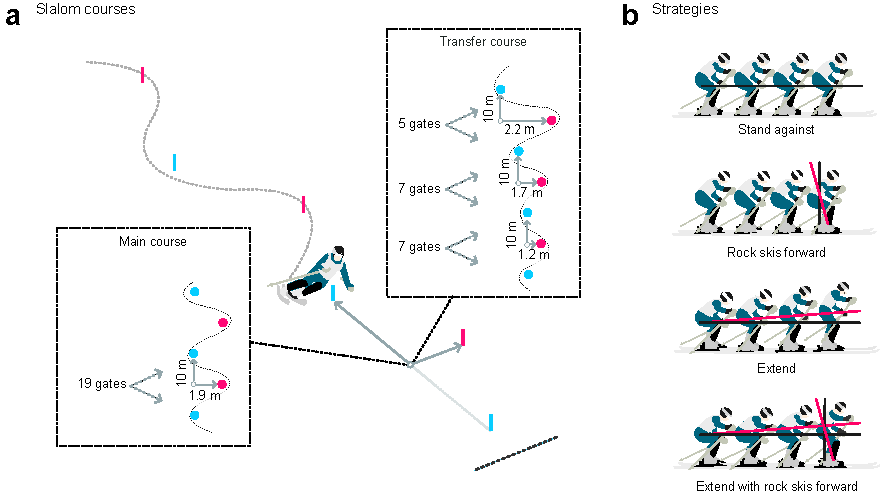
\includegraphics{figures/figure_method_courseandstrategy.pdf}
\caption{\textbf{a.} Illustrations of the two slalom courses used in the study. The main slalom course was a rhythmic course deployed in all sessions except for the transfer test. The course setting for the transfer test involved a progression in gate offset, starting with the largest offset and ending with the smallest offset. \textbf{b.} Illustration of the strategies defined to enhance racing performance on flat terrain in slalom: The "stand against" strategy emphasized maintaining a stable stance against external forces without body extension along the body's longitudinal axis or rocking skis forward; 'Rock skis forward' involved rocking skis forward from gate passage to completion of the turn; The "extend" strategy involves extending the body from a laterally tilted position during the turn, closer to the turn's center of rotation; The "extend with rocking skis forward" was expected to be the best strategy combining the two effects from extending and rocking skis forward, and we therefore defined this as the theoretical best strategy}
\label{fig:courseandstrategies}
\end{figure}

\begin{figure}[H]
\centering
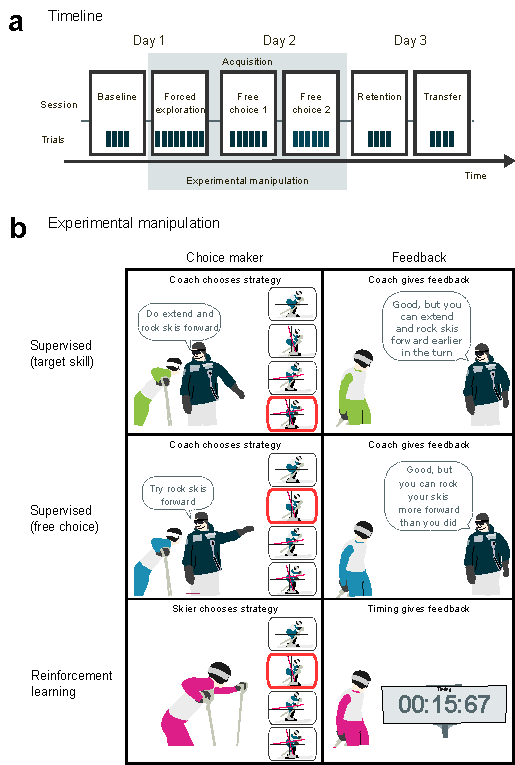
\includegraphics{figures/figure_method_experiment.pdf}
\caption{Illustration of the experimental design and procedure. \textbf{a.} Timeline of the three-day learning experiment. During the baseline, skiers skied a slalom course in the shortest amount of time possible without receiving race time feedback. The skiers were then assigned to three treatment groups (see b). In their assigned group, skiers underwent an acquisition phase in their designated treatment group comprising one Forced Exploration (skiers performed all strategies) and two Free Choice sessions (skiers or coaches could choose strategies themselves). On the last day, skiers completed a retention and transfer test where they could pick strategy themselves, again without receiving race time feedback. \textbf{b.} Illustration of treatment groups in the study. Supervised (target skill) learning involved coaches consistently choosing the theoretically best strategy (except during Forced Exploration), while supervised (free choice) learning allowed coaches to freely select strategies. Skiers in both of these treatment groups received feedback on strategy execution from their respective coach, while skiers in the reinforcement learning group independently selected strategies and received feedback from the timing system to facilitate value learning of each strategy}
\label{fig:experiment}
\end{figure}

\section{Method}


\subsection{Participants}
Conducting studies on alpine ski racing poses challenges related to environmental control and resource constraints. Our sample size approach involved recruiting as many skiers as possible during June 2023, when we had a short time window to test skiers in the indoor ski hall. We set the minimum sample size to 80 skiers, which we deemed appropriate for this context. Prior to data collection, data and power simulations for sample sizes of 80, 100, and 120 skiers were conducted, revealing simulated powers of 0.60, 0.75, and 0.80, respectively, for the smallest effect size of interest (0.3 second difference between groups) (\url{https://osf.io/c4t28}). The smallest effect size of interest was based on our knowledge of alpine skiing and discussions with coaches, but it was intended for a 50-meter longer course and more training sessions than we ultimately ended up using due to practical considerations. We deliberately opted to recruit skiers with diverse skill levels for the study to augment the generalizability of our findings. However, to ensure a sufficient skill level to handle the specific icy snow conditions prepared in the skiing hall, we recruited only skiers aged 15 and older. The sample size justification, task design, and analysis plan were preregistered before data collection (\url{https://osf.io/tfb2w}).

We managed to recruit ten alpine ski teams comprising 98 alpine ski racers from Norway and Sweden (age M = 18.1 years, SD= 2; 40 females, 58 males). Two skiers were excluded from the analysis due to an injury prior to the study (n=1) or sickness during the study (n=1); thus, a total of 96 skiers completed the entire study and were included in the analysis.  Among the ski groups tested were five ski academies, three senior development teams, and two national ski teams. These skiers were generally highly skilled, with a median world rank of 605, but there was also considerable variability, as indicated by a substantial interquartile range (Q1 = 248, Q3 = 1390.5). A smaller subset of the participants (n = 13) were not world-ranked,  as they had yet to compete in internationally sanctioned races that form the basis for calculating athlete points and rankings. Table 1 provides demographic information for each treatment group.

We also recruited 11 coaches (2 women; 6 men) to serve as coaches for the supervised learning groups. This selection was pragmatic because it was not possible to test all ski teams simultaneously due to space and time constraints in the skill hall. The 10 ski teams were therefore divided into 4 groups for which the study was conducted at different times. For each of the four groups, we recruited two coaches from the ski teams to serve as coaches in the supervised (free choice) learning group, totaling 8 coaches (2 women; 6 men). These coaches had extensive coaching experience in coaching alpine ski racers. In addition, for each group of ski teams that completed the experiment together, we recruited a third coach to coach the skiers in supervised (target skill) learning. To ensure that these coaches had sufficient credibility to make the skiers buy into our theoretical best strategy, we selectively recruited three highly experienced coaches from the Norwegian alpine ski team (one coach had to serve twice due to illness of the fourth coach). Importantly, all the coaches remained unaware of the experimental manipulation. Table \ref{descriptive_coach} provides demographic information about the coaches. All the skiers and coaches provided informed consent before the study. The study was approved by the Human Research Ethics Committee of The Norwegian School of Sport Sciences.


\begin{sidewaystable}
\label{descriptive_skier}
\caption{\textbf{Skier characteristics}}
\centering
\begin{tabular}[H]{l|c|c|c|c|c|c}
\hline
\multicolumn{1}{c|}{ } & \multicolumn{2}{c|}{\textbf{Reinforcement learning}} & \multicolumn{2}{c|}{\textbf{Supervised (free choice)}} & \multicolumn{2}{c}{\textbf{Supervised (target skill)}} \\
\textbf{Sex} & \textbf{F}, N = 13 & \textbf{M}, N = 19 & \textbf{F}, N = 14 & \textbf{M}, N = 19 & \textbf{F}, N = 13 & \textbf{M}, N = 20\\
\hline
Age & 18.4 (2.3) & 17.7 (1.8) & 18.1 (2.3) & 18.3 (1.8) & 17.8 (2.4) & 18.2 (2.1)\\
\hline
Training group &  &  &  &  &  & \\
\hline
\hspace{1em}National team & 1 (7.7\%) & 1 (5.3\%) & 2 (14\%) & 1 (5.3\%) & 2 (15\%) & 4 (20\%)\\
\hline
\hspace{1em}Senior team & 3 (23\%) & 5 (26\%) & 1 (7.1\%) & 5 (26\%) & 0 (0\%) & 5 (25\%)\\
\hline
\hspace{1em}Ski academy & 9 (69\%) & 13 (68\%) & 11 (79\%) & 13 (68\%) & 11 (85\%) & 11 (55\%)\\
\hline
FIS points &  &  &  &  &  & \\
\hline
\hspace{1em}Median (IQR) & 54 (42, 80) & 46 (34, 90) & 58 (26, 80) & 44 (35, 61) & 49 (28, 66) & 31 (28, 63)\\
\hline
\hspace{1em}Not recorded & 3 & 2 & 1 & 2 & 2 & \vphantom{1} 3\\
\hline
World ranking &  &  &  &  &  & \\
\hline
\hspace{1em}Median (IQR) & 630 (394, 1,217) & 707 (364, 2,317) & 709 (133, 1,224) & 662 (387, 1,274) & 527 (145, 882) & 314 (220, 1,360)\\
\hline
\hspace{1em}Not recorded & 3 & 2 & 1 & 2 & 2 & 3\\
\hline
\multicolumn{7}{l}{\rule{0pt}{1em}\textsuperscript{1} Mean (SD); n (\%)}\\
\end{tabular}
\end{sidewaystable}


\begin{sidewaystable}\label{descriptive_coach}
\caption{\textbf{Coach characteristics}}
\centering
\begin{tabular}[H]{l|c|c|c}
\hline
\multicolumn{1}{c|}{ } & \multicolumn{2}{c|}{\textbf{Supervised (free choice)}} & \multicolumn{1}{c}{\textbf{Supervised (target skill)}} \\
\textbf{Characteristic} & \textbf{F}, N = 2 & \textbf{M}, N = 6 & \textbf{M}, N = 3\\
\hline
Age & 38.5 (3.5) & 44.3 (8.8) & 48.0 (7.0)\\
\hline
Ski education (highest achieved) &  &  & \\
\hline
\hspace{1em}Level 2 & 0 (0\%) & 1 (17\%) & \\
\hline
\hspace{1em}Level 3/4 & 2 (100\%) & 5 (83\%) & 3 (100\%)\\
\hline
Sport science degree (highest achieved) &  &  & \\
\hline
\hspace{1em}MSc & 1 (50\%) & 0 (0\%) & 1 (33\%)\\
\hline
\hspace{1em}BSc & 1 (50\%) & 1 (17\%) & 1 (33\%)\\
\hline
\hspace{1em}No & 0 (0\%) & 4 (67\%) & \\
\hline
\hspace{1em}One-year program & 0 (0\%) & 1 (17\%) & 1 (33\%)\\
\hline
Coaching experience (years) &  &  & \\
\hline
\hspace{1em}National team (WC/EC)/Senior teams & 5.00 (1.41) & 5.00 (4.24) & 15.67 (1.15)\\
\hline
\hspace{1em}Ski academy & 7.5 (3.5) & 7.5 (6.5) & 2.00 (3.46)\\
\hline
\hspace{1em}Ski club & 2.5 (3.5) & 6.5 (8.7) & 6.0 (6.6)\\
\hline
\multicolumn{4}{l}{\rule{0pt}{1em}\textsuperscript{1} Mean (SD); n (\%)}\\
\end{tabular}
\end{sidewaystable} 


\subsection{The setup}
The experiment was conducted in the indoor ski hall SNØ in Oslo, Norway (\url{https://snooslo.no/}). In this hall, we used a 210-meter-long flat section of the race hill, which we water-injected before testing each group of skiers to ensure uniform and fair snow conditions for all skiers (Supplementary \ref{sup_snowprep} for detailed description). With our chosen course setup, this 210-meter-long flat section allowed space for 19 slalom gates. 

We used two types of slalom courses in the experiment (Fig. \ref{fig:courseandstrategies}a). The main slalom course was used in all sessions, except during the transfer test, and featured a 10 m distance and a 1.9 m offset. The course distance aligned with our previous study \cite{magelssen_is_2022}, but we opted for a slightly larger offset to better suit the skill level of our skiers. The transfer test evaluated how well the skiers transferred their learning to a new slalom course more realistic to a typical alpine ski race course. To assess this, we set a course with a progression in gate offset, starting with five gates at a 2.2-meter offset, followed by seven gates at a 1.7-meter offset, and concluding with seven gates at a 1.2-meter offset. Although we did not expect radical differences in strategy effects, we anticipated a greater emphasis on rocking the skis forward in gates with a 2.2-meter offset than in those with a 1.2-meter offset to enhance turn exit release. Both courses were set with stubbies (short gates) instead of long gates to minimize energy dissipation upon hitting the gate \cite{minetti_biomechanics_2018}. Using long gates can also be a distracting element in that skiers' attention is allocated to clearing the gate instead of focusing on executing the skill. Finally, this approach helped us avoid creating holes in the course, which can occur when the long gate is forcefully slammed into the ground. To minimize wear and tear on the course, we set two parallel and identical courses and routinely shifted between them.

The start gate was positioned 20 meters before the first gate. Skiers were required to start in a static position to ensure consistency in the starts, with their binding front head placed behind the starting gate. The skiers started by putting their skis in parallel and lifting the poles without using poling or skating for propulsion (Supplement Video illustrates the starting procedure and setup). We recorded the times using a wireless photocell timing system (HC Timing wiNode and wiTimer; Oslo, Norway). Timing started when the skier crossed the first photocell pair situated 10 meters below the starting gate. 
 
\subsection{Experimental design}
We employed a between-subjects design and posed the learning question of discovering effective strategies as an \textit{n}-armed bandit problem \cite{sutton_reinforcement_2018}. The essence of this problem is that a learner repeatedly tries different options and observes their outcomes to learn which strategy is the best and, therefore, which one to choose. Finding the best strategy requires a delicate balance between exploiting the strategy known to yield the best payoff and exploring alternative strategies that may offer superior benefits. In our study, the options consisted of four strategies that skiers could employ to improve their race times on flat slopes in slalom, grounded in physics-based coaching manuals for alpine ski racing \cite{lemaster_skiers_1999, lemaster_ultimate_2010, lind_physics_2013}, biomechanical research on elite skiers \cite{reid_kinematic_2010, reid_alpine_2020, magelssen_is_2022}  or common strategies used by coaches.  The four strategies were named "stand against", "rock skis forward", "extend", and "extend with rock skis forward (see Fig.\ref{fig:courseandstrategies}b for a strategy illustration and Supplementary\ref{sup_strategies} for an extended explanation). To study how instruction and feedback drive learning in strategy selection, we designed and allocated skiers to three treatment groups, which allowed us to compare reinforcement learning with traditional supervised learning with a coach: 

For the supervised (target skill) learning group, we provided the best possible training program by engaging highly experienced and meritorious coaches who explained to the skiers that the 'extend with rock skis forward' strategy was the most effective for skiing fast on flat terrain in slalom. They provided this information, citing a previous doctoral project \cite{reid_kinematic_2010}, which revealed that the fastest slalom racers spent more time aft of the skis, emphasizing the involvement of a dynamic rocking movement. In addition, the coaches reported that simulations of ski racers yielded similar results. In addition, the coaches reported that simulations of ski racers yielded similar results \cite{mote_accelerations_1983, lind_physics_2013}. The coach then instructed the skiers to adopt this strategy and provided feedback on its execution after each trial. Note that the coach had access to the skiers after each trial but was prohibited from sharing this information with the skiers.

In the supervised (free choice) learning group, skiers were assigned to two coaches recruited from the tested group of ski teams. We recruited two coaches to minimize waiting time and thus enhance training efficiency. To balance the skiers' skill levels between the two coaches, we created new blocks from the ranked list from baseline testing and randomly assigned them to the coaches. We instructed the coaches to improve the skiers' race times as much as possible with our four defined strategies to their disposal to achieve this goal. For each trial, the coach selected a strategy for the skier, observed the skier during his trial and provided feedback on its execution afterward. Similar to the supervised (target skill) learning group, the coaches had access to the skiers' data after each trial but could not share this information with the skiers.

In contrast, the reinforcement learning group was not assigned to any coach. Instead of having a coach deciding the skiing strategy for them, the skiers in this treatment group were told to choose a strategy for each trial by themselves to ski the course as fast as possible. To help the skiers choose and learn from evaluation, this group could see their racing times immediately after they crossed the finish line. Although this group had no coach, we assigned a person to communicate with the skiers to record their choices and encourage them to try skiing quickly to prevent boredom effect.

\subsection{Procedures}\label{subsec4}
Figure \ref{fig:experiment}a illustrates the procedures employed in the study. 
In the baseline test, skiers began with two warm-up runs: one in free skiing warm-up course and one specific warm-up in the slalom course. During these warm-up runs, skiers were instructed, trained and verified on the start procedure and start technique by an instructor. As a first run in the baseline assessment, skiers completed a straight-gliding run, where they skied straight down from start to finish in a static, upright slalom posture. Subsequently, the skiers completed four runs in the slalom course. Skiers were encouraged to ski as quickly as they could, but they could not see their times, nor did they get any instruction on how to perform well. 

After the initial baseline assessment, the skiers took a 60-minute break. In the meantime, we allocated the skiers to the three treatment groups: reinforcement learning, supervised learning (target skill), and supervised learning (free choice). To allocate the skiers to groups, we deployed a randomized-blocked approach to account for pre-existing differences in the skiers’ performance levels \cite{maxwell_designing_2017}. Specifically, we computed each skier’s average performance across the four trials in the baseline and ranked them accordingly. We then created \textit{n} blocks with block sizes corresponding to our three treatments for the entire list of skiers and assigned these skiers to these predefined blocks. Finally, we randomly allocated the skiers to the different treatment groups within each block (Figure \ref{fig:experiment}b).

The treatment groups participated in sessions at different times to prevent treatment diffusion \cite{maxwell_designing_2017}. As the ski group comprised teams of skiers who know each other well and were residing together, we explicitly emphasized the importance of keeping information about the sessions private. To stay within the time frame at the ski hall, the two supervised learning groups underwent training together. To facilitate this, we arranged stations in the finish area with space and vision dividers and ample space to impede communication between coaches in the supervised learning groups (Supplementary \ref{fig:coachstation}). In addition, we developed a Python script that fetched racing times from the timing system, filtered the times for each coach, and transmitted it to the station where the coach was located, ensuring no information leak between coaches. The treatment group that initiated after the baseline session was randomized and counterbalanced across the group of ski teams we tested.

The first session after the treatment assignment involved a forced exploration. Here, skiers within the treatment group were gathered, and the session started by introducing them to the strategies. We explained that we had identified four strategies to enhance racing times on flats in slalom. Subsequently, each strategy was detailed, supported by illustrative drawings in \ref{fig:courseandstrategies}b Figure and corresponding word explanations as outlined in the \ref{subsec4}. To confirm comprehension, we conducted two short familiarization trials for each strategy, or until the execution met our performance standards. After reviewing the strategies with the participants, we gathered them in their respective treatment groups and asked them to rank the strategies online for what they believe are most to least suitable to improve performance in flat terrain slalom skiing. Throughout the instruction and ranking process, skiers were explicitly instructed not to discuss the strategies with each other. It is important to note that the same instructor was used for all treatment groups within a tested ski group. After this, the skiers conducted a total of eight trials on the course, with two trials for each strategy. During these trials, the reinforcement learning group got feedback from the timing whereas the coach gave feedback in the supervised learning. After completing the eight rounds, the skiers re-evaluated and ranked the strategies.

On the second day, skiers completed two free-choice sessions, each comprising a total of 6 trials in the same slalom courses that were used the baseline testing the day before. Prior to the 6 free - choice trials, the skiers performed one warm-up free skiing run and one warm-up run in the slalom course. In these sessions, supervised (target skill) learning consistently selected the theoretically best skiing strategy. Conversely, in supervised (free choice) and reinforcement learning, the coach and the skiers, respectively, had the autonomy to choose skiing strategy for each run. After each session, coaches (except supervised target skill) and skiers were asked to re-evaluate and rank the strategies.

On the third and last day, the skiers performed a retention and a transfer test to assess the effect of the training approaches on learning and performance. The retention test was performed in the same course as the baseline and acquisition sessions, whereas the transfer test was performed in the transfer course and involved a progression in gate offset from start to finish. Since the transfer test was a new course, we allowed the skiers to inspect the course before the test. The retention and transfer tests were conducted with all treatment groups together. None of the treatment groups received any feedback from coaches nor time during these tests. After each test, the skiers were asked to rank the strategies. 

\subsection{Analysis}
The data were cleaned with custom functions built on tidyverse \cite{wickham_welcome_2019} packages in R. After this process, we validated the data by performing trial counting and visual inspection of the race time to screen for errors. An extensive report of this cleaning and validation process can be found at OSF  (\url{https://osf.io/2jxgk}).

Due to the hierarchical structure of the data, our general statistical strategy relies on multilevel modeling. At the first level, each skier performed multiple trials during each session. At the second level, each skier was nested within groups of ski teams that performed the experiment together. To account for these multilevel data structures, we leveraged linear mixed-effects models. To model random effects, we adopted a design-driven approach \cite{barr_random_2013, barr_learning_2021}, where we sought to account for all nonindependence introduced by repeated sampling from the same ski group and skier. We deployed classical frequentist statistics and fitted these models with the lme4 package \cite{bates_fitting_2015} in the R programming language. We used a simple coding scheme for our predictors where the intercepts represent the estimated mean of the cell means and the contrasts represent the estimated difference with respect to the reference level, which we set for reinforcement learning. Two-tailed p values and degrees of freedom for each model were derived using the lmerTest package \cite{kuznetsova_lmertest_2017} via the Satterthwaite approximation method. Alpha was set to 0.05 for all test statistics.

 \subsubsection{Race time}

Race time was analyzed using linear mixed-effect regression models. Initially, we planned to normalize the racing time by expressing the racing time as the difference from the straight-gliding time performed at the beginning of every session. This difference better approximate the skiers' actual skill improvement by considering the variance in snow conditions. However, practical considerations led us to deviate from this approach. This change was necessary because we had to flip or shift the course after each day to ensure snow conditions with the least damage. Unfortunately, these adjustments made maintaining a clean, straight-gliding lane difficult since the straight gliding lane crossed many areas with damage to the snow surface (holes) from the previous course set (see \ref{sup_coursesetting} for an image of these holes). Collisions with these holes affected the race time, adding noise to the results. Therefore, we used a more conservative approach and analyzed the raw racing times instead of analyzing the normalized racing times.

For the acquisition session, we modeled race time using Session and Treatment, and their interactions, as predictors. For retention and transfer, we modeled racing times at these sessions, with treatment added as a predictor. In addition, we used the average performance for each skier on the baseline test as a predictor to improve estimate precision and adjust for group differences at baseline testing. 

To model the effect and development of the strategies we broke the analysis up into different sub-models. One analysis focused on differences in the strategies and groups regarding Forced Exploration, where all participants had completed all strategies. Another analysis examined the transition from Forced Exploration to retention for both supervised (free choice) and reinforcement learning. The final model investigated the development between groups specifically for the "extend with rock skis forward" strategy. Session was coded as a continuous variable in all models. 


\subsubsection{Strategy choices}

Strategy choices were analyzed using generalized linear mixed-effect regression models with a binomial logit-link function. To model the selection of the theoretical best strategy, we inputted the data as logistic, where for each trial (\(i\)) per skier (\(j\)) within ski group (\(k\)), we counted \(y_{ijk}=1\) when the skier chose the theoretical best strategy (that is, 'extend with rock skis forward') or 0 when they did not. We included Treatment and Session and their interaction as two variables. To account for the nonindependence of the data structure, we allowed the intercept to vary by including a random intercept for the skier and ski groups.

We adopted the same model formula to model the selection of the estimated best strategy. This time, however, we counted \(y_{ijk}=1\) when the skier chose their estimated best strategy and 0 when they did not select that strategy. To estimate the best strategy for each skier in the sample, we used the sample-average method \cite{sutton_reinforcement_2018} to average the race time for each strategy and selected the strategy with the lowest estimated (that is, best) value. The sessions that we used to form this average were Forced Exploration, Free Choice 1, and Free Choice 2.  Due to the scaling issues with generalized linear models, we followed the recommendation to determine the size and significance of the effects of interest using marginal effects on the probability scale \cite{mize_best_2019, mccabe_interpreting_2022}. Interactions were assessed using discrete difference (also second difference), which is also in line with these recommendations. To derive these estimates, we used the emmeans package \cite{lenth_emmeans_2023}.

\subsubsection{Sensitivity to feedback}

To learn how skiers and coaches used feedback to guide their choices, we constructed a 'win-stay, lose-switch' model (WSLS; \cite{nowak_strategy_1993, worthy_comparison_2014, iyer_probing_2020}). For this WSLS analysis, we z-scored the race times for each skier for Free Choices 1 and 2 and counted \(y_{ijk}=1\) when the skier repeated the previous strategy and 0 when it was not. The data were modeled using a generalized linear mixed-effect regression model with a binomial logit-link function, with Treatment and z-transformed Race Time and their interaction as the two variables. To test for differences in error sensitivity, we used the marginal effects at the mean (MEM) derived from the emmeans package \cite{lenth_emmeans_2023}.


\subsubsection{Evaluations of the strategies}
To analyze the strategies' rankings, we used single-level linear regression owing to the singularity of our multilevel models. In this model, we inputted Session as a continuous variable and Treatment as the predictors. For supervised (free choice) learning, we used the coaches' rankings during the sessions where they selected strategies, and we used the skiers' rankings when they selected strategies during the retention and transfer tests .



\section{Results}


\subsection{Race time}\label{result_racetime}
We posited that strategy choice would greatly impact race time in the slalom course and that the reinforcement learning group would learn to select better strategies and consequently perform better over the course of the experiment compared to the two supervised learning groups. As our first step in the analysis, we assessed whether there were pure time differences between the groups across the different sessions without taking the chosen strategy into account. 

If reinforcement learning were to learn to select better strategies, we would expect to observe differences in improvement among the three learning groups over the course of the three acquisition sessions. Therefore, our hypothesis was that the reinforcement learning group would improve more during the acquisition sessions than the two supervised learning groups. Initially, we found no statistically significant differences between the reinforcement learning group and the supervised (free choice) learning group ($\beta$ = 0.06 , 95\% CI [-0.2, 0.32], $t$(92.727) = 0.48, $p$ = 0.631) ) or between the supervised (target skill) learning group ($\beta$ = 0.18, 95\% CI[-0.08, 0.44], $t$(92.663) = 1.37, $p$ = 0.174) during the first acquisition session (forced exploration). This finding was expected, however, since all groups had the same number of trials on each strategy in this session. By contrast, we would expect differences in improvement over the course of the second (free choice 1) and third (free choice 2) acquisition session, when the skiers or the coach had the autonomy to pick strategy. We found that all treatment groups significantly improved their race times over the course of the free choice sessions during acquisition (Supplementary Table \ref{table_racetime_acquisition_change}), suggesting that the choice of strategy influenced the race time. The rate at which they improved, however, differed across the three groups during the two sessions: supervised (target skill) learning showed a statistically significant greater improvement than reinforcement learning from forced exploration to free choice 1 when skiers were solely coached to select the theoretically best strategy ($\beta$ = -0.12, 95\% CI[-0.22, -0.03], $t$(91.777) = -2.58, $p$ = 0.012). Conversely, supervised (free choice) learning demonstrated a descriptively poorer progression than reinforcement learning, albeit the difference was not statistically significant ($\beta$ = 0.08, 95\% CI[-0.02, 0.17], $t$(92.5) = 1.61, $p$ = 0.110). This difference, however, became significant by the final acquisition session (Free Choice 2) ($\beta$ = 0.14, 95\% CI[0.02, 0.26], $t$(95.743) = 2.26, $p$ = 0.026). Supervised (target skill) learning showed a descriptive decline from Free Choice 1 to Free Choice 2, attenuating that their initially greater improvement rate relative to reinforcement learning became statistically nonsignificant  ($\beta$ = 0.02, 95\% CI[-0.11, 0.14], $t$(95.651) = 0.26, $p$ = 0.798). We did not, however, find statistical evidence that reinforcement learning performed better than supervised (free choice) or supervised (target skill) learning at Free Choice 1 or Free Choice 2 (Supplementary Table \ref{table_racetime_acquisition_groupdifference}). 

In the retention session, skiers independently chose their strategies, irrespective of their assigned groups.  Our hypothesis was that reinforcement learning would outperform the two supervised learning groups in retention due to better strategy selection learned from observing the race times to evaluate the strategies . Fig. \ref{fig: racetime}b presents the mean race time estimates during retention. We found that the race times for the reinforcement learning group were on average significantly better than those for supervised (free choice) learning, when controlling for baseline differences ($\beta$ = 0.12, 95\% CI[0.01, 0.24], $t$(101.422) = 2.12, $p$ = 0.037). The difference between reinforcement learning and supervised learning (target skill) also favored reinforcement learning but was smaller and not statistically significant ($\beta$ = 0.07, 95\% CI[ -0.04, 0.19], $t$(101.63) = 1.27, $p$ = 0.206). We therefore provide evidence that reinforcement learning performed better at retention than supervised (free choice) learning but not significantly better than supervised (target skill) learning. 

We also hypothesized that reinforcement learning would improved skill transfer to a new slalom course. Fig. \ref{fig: racetime}c presents the mean race time estimates during Transfer. As for retention, the race time on the transfer course was on average better in reinforcement learning than in supervised (free choice), yet the difference was smaller and not statistically significant, when controlling for baseline differences ($\beta$ = 0.1, 95\% CI[-0.02, 0.21], $t$( 99.979) = 1.7, $p$  = 0.091). The race times for reinforcement learning and supervised (target skill) learning was on average identical when controlling for baseline differences ($\beta$ = 0, 95\% CI[-0.12, 0.11], $t$(100.033) = -0.04, $p$ = 0.967). Thus, we did not find corroborating evidence for improved transfer.



\begin{figure}[H]
\centering
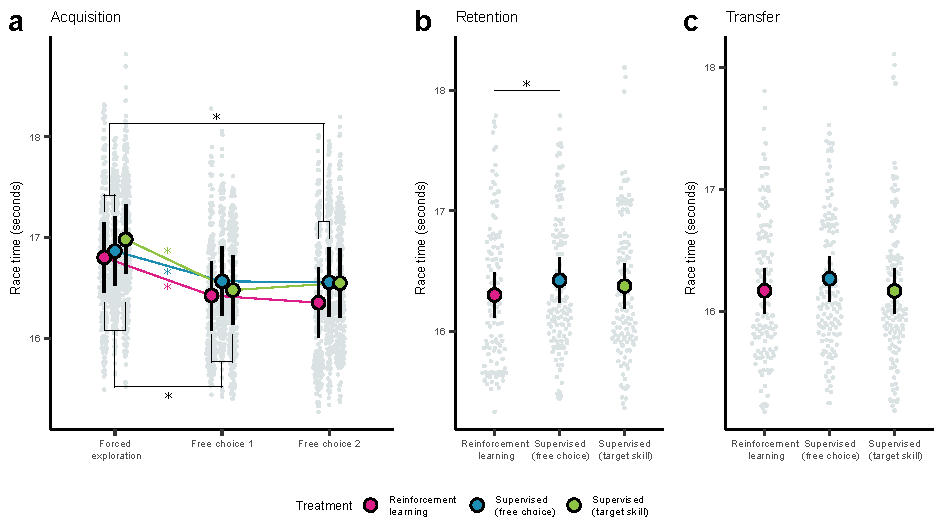
\includegraphics{figures/figure_racingtimes_2.pdf}
\caption{Race time across the different sessions for the three treatment groups. \textbf{a}. Displays the estimated race time during the three acquisition sessions. Forced Exploration refers to the sessions wherein skiers tried all strategies, whereas Free Choice 1 and Free Choice 2 refer to the session wherein skiers or coaches selected strategies according to their assigned treatment groups. \textbf{b.} Displays the estimated race time for retention. \textbf{c.} Displays the estimated race time for Transfer. Intervals represent the 95\% Confidence Interval (CI) derived from the models. Asterisks (*) indicate a statistically significant effect. Each light gray point represents a single trial performed by a skier, thus showing the full multilevel structure of the dataset}
\label{fig: racetime}
\end{figure}


\subsection{Strategy choices}\label{result_strategychoice}
We proposed that the differences in race time between the groups could be explained by the choice of strategy. Specifically, we hypothesized that reinforcement learning would learn to choose better strategies than supervised learning groups by learning the strategies' values directly from observing race times. Fig. \ref{fig: choice_descriptives} displays the percentage selections of the four strategies across all sessions.


\begin{figure}[H]
\centering
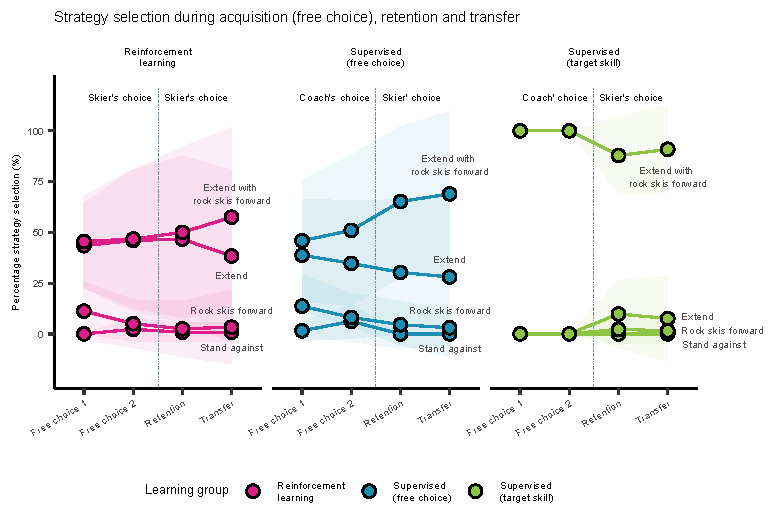
\includegraphics{figures/figure_choice_descriptivecount_4.pdf}
\caption{Descriptive strategy choices for skiers in each session, with bars indicating percentages and the numbers to the right of the bars showing the total count for
each strategy}\label{fig: choice_descriptives}
\end{figure}


We first assumed that our theoretically defined best strategy was indeed the best strategy and tested whether reinforcement learning had a greater probability of selecting this strategy than supervised (free choice) learning. Note that supervised (target skill) learning was excluded from this analysis because only this strategy was selected. Fig. \ref{fig: choice_estimated}a displays the predicted probabilities for the treatment groups across the four sessions where the skiers or coaches were given autonomy to select strategy themselves. We found that both groups showed a statistically significant increase in the probability of choosing the strategy we considered theoretically optimal across the four sessions (Supplementary Table \ref{strategychoice_theorybest_change}); however, the timing of this increase differed between the two groups. For supervised (free choice) learning we found a statistically significant increase from free choice 1 to retention, when skiers in this group were given autonomy to choose strategies themselves (0.31, 95\% CI[0.18, 0.44], $z$ = 4.59, $p$ < 0.001). This probability increase was significantly greater than the increase for reinforcement learning (0.24, 95\% CI[0.05, 0.43], $z$ = 2.43 , $p$ = 0.015), which did not significantly increase from free choice 1 (0.07, 95\% CI[-0.07, 0.21], $z$ = 0.96, $p$ = 0.339). Reinforcement learning, on the other hand, significantly increased the probability of choosing the theoretically best strategy in the transfer session relative to free choice 1 (0.18, 95\%CI[0.04, 0.32], $z$ = 2.58, $p$ = 0.010). Despite the descriptively higher probability of choosing the theoretical best strategy in supervised (free choice) learning during the free choice 2, retention and transfer sessions, none of the differences between the groups at each session were statistically significant (Supplementary Table \ref{strategychoice_theorybest_groupdiff}). 

\begin{figure}[H]
\centering
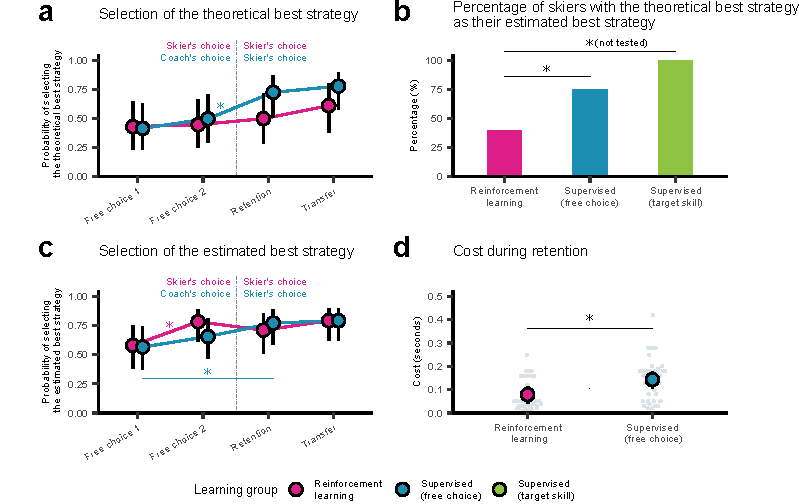
\includegraphics{figures/figure_choice_estimated_4.pdf}
\caption{Strategy selection for reinforcement learning (pink) and supervised (free choice) learning (blue) during acquisition. \textbf{a.} Displays the predicted probability of choosing the theoretically best strategy (that is, 'extend with rocking skis forward') for both reinforcement learning and supervised (free choice) learning. \textbf{b.} Displays the predicted probability of selecting the individual skier's estimated best strategy using the sampling averaging method\cite{sutton_reinforcement_2018}. Intervals represent the 95\% confidence intervals (CIs) derived from the models. Asterisks (*) indicate a statistically significant effect}\label{fig: choice_estimated}
\end{figure}

The previous analysis revealed no evidence of a higher probability of selecting what we defined as the theoretically optimal strategy in reinforcement learning. Instead, the descriptive trend favored supervised (free choice) learning. We therefore wondered whether there was a greater proportion of skiers in the supervised (free choice) learning group whose theoretically best strategy corresponded to their own estimated best strategy, and performed a follow-up analysis to test this possibility. Fig.\ref{fig: choice_estimated}b shows the proportion of skiers for each group that had the theoretical best strategy as their estimated best strategy. Overall, 75\% of the skiers in supervised (free choice) learning had the theoretically best strategy as their estimated best strategy compared to only 40\% in the reinforcement learning group. A chi-square test revealed a statistically significant association between groups $\chi^2$ = 6.42, $p$ = 0.01). Because all skiers in the supervised (target skill) group had the theoretical best as their estimated best strategy (see Fig.\ref{fig: choice_estimated}b), they could not be included in this analysis. More skiers in the supervised (free choice) learning group had the theoretically best strategy as their estimated best strategy, which can explain why they had a descriptively higher probability of choosing it compared to reinforcement learning.

What we defined as the theoretical best strategy may not have been the optimal strategy for each individual skier, however. Next, we tested whether reinforcement learning had a greater probability of selecting the individual skiers' estimated best strategy.  Fig. \ref{fig: choice_estimated}c displays the predicted probabilities of choosing the estimated best strategy for the treatment groups across the sessions. During the first session, in which we allowed skiers and coaches to choose their own strategies (free choice 1),  we found no statistically significant differences between the groups (0.01, 95\% CI[-0.22, 0.24], $z$ = 0.12, $p$ = 0.904). Both groups significantly improved their choices over the course of the sessions relative to free choice 1 (Supplementary table \ref{table_strategychoice_estimatedbest_change}), but the significant improvement came at different time points. We found a statistically significant improvement in choice for reinforcement learning from free choice 1 to free choice 2 (0.2, 95\% CI[0.09, 0.32], $z$ = 3.39, $p$ < 0.001), which was not statistically significant for supervised (free choice) learning (0.09, 95\% CI[-0.03, 0.21], $z$ = 1.48, $p$ = 0.140). However, the greater increase in the probability of choosing this strategy in reinforcement learning was not significant (0.11, 95\% CI [-0.28, 0.05], $z$ = -1.33, $p$ = 0.184). For supervised (free choice) learning we found a statistically significant improvement in their choices when the skiers made their own strategy choices during retention (0.21, 95\% CI[0.08, 0.34], $z$ = 3.11 , $p$  =  0.002). We found no statistically significant differences between the groups in any of the sessions (Supplementary table \ref{table_strategychoice_estimatedbest_groupdiff} ). We therefore did not find corroborating evidence that reinforcement learning learned to pick the best strategy more often than supervised (free choice) learning. 

Making good choices can extend beyond the mere selection of an optimal strategy, however. At times, multiple strategies yield outcomes that are closely similar, affording the learner to choose any without compromising performance. The task then becomes one of selecting strategies that offer comparable outcomes while avoiding those that carry the risk of substantially worse performance. We reasoned that discerning differences between fairly similar strategies could be tricky for skiers due to small time differentials that are influenced by noise, such as hitting a bump in a gate. Consequently, two or more strategies may appear nearly identical and be difficult for skiers to distinguish. We reasoned that reinforcement learning had learned to select good strategies that all led to nearly similar good outcomes and learned to steer away from those that led to poor outcomes. In a follow-up analysis, we calculated the expected difference between a skier's chosen suboptimal strategy and their estimated best strategy, which we termed 'cost.' This analysis revealed that reinforcement learning had significantly lower costs during retention than supervised (free choice) learning did  ($\beta$ = 0.06 , 95\% CI [0.01, 0.12], $t$(30.789) = 2.55 , $p$ = 0.016). This suggests that skiers in the reinforcement learning group may have learned to select better strategies, although we did not find evidence that they had a greater probability of picking the best strategy.

Finally, we examined the extent to which decision-makers (skiers in reinforcement learning and coaches in supervised learning) engaged with their feedback times to inform decisions about which strategy to adopt. Our hypothesis was that, compared with coaches, reinforcement learning would engage more actively with these race times to make optimal choices. To test this hypothesis, we conducted a 'win-stay, lose-switch' (WSLS) analysis, where the primary assumption is that all information used for decision-making stems from the last trial (k-1). In this analysis, heightened sensitivity is reflected by a high predicted probability of repeating an action following positive feedback and a low predicted probability following negative feedback on the preceding trial. Figure \ref{fig: choice_wsls} shows the predicted probability of repeating the strategy on the previous trial if the feedback was good. We found statistically significant estimated marginal effects at the mean (MEM) for both reinforcement learning  (-0.18, 95\% CI[-0.26, -0.11], $z$ = -4.8, $p$ < 0.001) and supervised (free choice) learning (-0.11, 95\% CI[-0.17, -0.04], $z$ = -3.29, $p$ $<$ 0.001). These findings suggest that both groups had a higher predicted probability of repeating a strategy if the previous trial feedback was good. Despite the large descriptive difference in the marginal effect between groups, this difference was not statistically  significant (-0.08, 95\% CI [-0.17, 0.02], $z$ = -1.55, $p$ $=$ 0.121). Thus, although we found that both groups were sensitive to feedback, we did not find evidence that reinforcement learning had greater sensitivity than supervised (free choice) learning. 

\subsection{Strategy evaluations and outcomes}
We also asked the skiers and coaches (excluding coaches involved in supervised (target skill) learning) to evaluate the strategies by ranking them from best (1) to worst (4) with the intention of directly assessing how their understanding of the strategies evolved and how this understanding governed their choices. They first ranked upon their introduction (familiarization) to the strategies and then after each session. Our hypothesis was that reinforcement learning would undergo distinct evaluations of the strategies compared to the supervised learning groups by having the race times at their disposal to evaluate the strategies. 

After the introduction to the strategies, but before the skiers had the chance to properly try out the strategies on the slalom course (familiarization), we found that the choice makers in all groups ranked 'extend with rock skis forward' as the best, followed by 'extend,' 'rock skis forward,' and 'stand against' (Supplementary Table \ref{table_strategyevaluation_diffstrategy} and Fig. \ref{fig: rank}a). We did not find any statistically significant difference between groups during this familiarization (Supplementary Table \ref{table_strategyevaluation_diffgroup}), with two exceptions: supervised (target skill) learning ranked 'extend' worse ($\beta$ = 0.45, 95\% CI[0.24,  0.67], $t$(1700) = 4.17, $p$ $<$ 0.001) and 'extend with rock skis forward' better  ($\beta$ = -0.42, 95\% CI[-0.63, -0.2], $t$(1700) = -3.83, $p$ $<$ 0.001) than reinforcement learning did.

Over the course of the sessions, we observed notable shifts in the average rankings of the strategies (Supplementary Table \ref{table_strategyevaluation_slopestrategy}a). The change was relatively flat and unchanged in terms of position for the worst ('stand against') and best ('extend with rock skis forward') strategies. However, we found that 'stand against' was ranked significantly worse ($\beta$ = 0.09, 95\% CI[0.04, 0.13], $t$(1700) = 3.4, $p$ $<$ 0.001)  and that 'extend with rock skis forward' was ranked significantly better ($\beta$ = -0.06 , 95\% CI[-0.11, -0.01], $t$(1700) = -2.51, $p$ = 0.012) over time in supervised (target skill) learning. Although reinforcement learning and supervised (free choice) learning followed the same trend, these trends were not statistically significant. More marked shifts were observed for the two middle-ranked strategies: 'extend' and 'rock skis forward'. Specifically, reinforcement learning ranked 'extend' significantly better  ($\beta$ = -0.1, 95\% CI[-0.15, -0.05], $t$(1700) = -3.73, $p$ < 0.001) and 'rock skis forward' significantly worse ($\beta$ = 0.09, 95\% CI [0.04, 0.15], $t$(1700) = 3.57, $p$ < 0.001) over the course of the sessions. Supervised (target skill) and supervised (free choice) also had the same trend, but the magnitude was smaller and did not reach statistical significance (Suppl table). We also found that there was a greater change in ranking of 'rock skis forward' in reinforcement learning group than in supervised (target skill) learning  ($\beta$ = -0.07, 95\% CI[-0.14 to 0], $t$(1700) = -1.97,$p$ = 0.049), suggesting a larger shift in strategy ranking for this ranking in reinforcement learning.  

These evaluations should also be linked to the race times for each strategy. It is possible, however, that different groups had different developments in the various strategies. Finally, we therefore tested whether different groups had different progressions in the various strategies. During the initial acquisition session when skiers tested all strategies (free choice 1), we found that all groups on average performed descriptively better with 'extend with rock skis forward', followed by 'extend', 'rock skis forward', and finally 'stand against'. We found no statistically significant differences between the reinforcement learning and supervised learning groups on any of these strategies. Because supervised (target skill) learning only performed 'extend with rock skis forward' during free choice 1 and free choice 2, we first built a model to test for differences in improvement on 'stand against', 'rock skis forward', and 'extend' only for reinforcement learning and supervised (free choice) learning. From this model, we found a statistical significant improvement in all strategies over the course of the sessions to retention, except for 'stand against' in reinforcement learning. This deviation, however, may be attributed to the limited number of observations for this strategy within the group. Interestingly, we found that the reinforcement learning group improved more on the "extend" strategy than the supervised (free choice) learning group ($\beta$ = 0.04 , 95\% CI[0.01, 0.07], $t$(1378.879) = 2.34, $p$ = 0.020). We did not find evidence for such an interaction effect for any of the other three strategies ( Supplementary Table \ref{Supplementarytable_strategyeffect_7}). Dette er et interessant funn fordi denne gruppen ikke hadde noen trener, men kun fikk se tidene. Til slutt, As supervised (target skill) learning only trained on the "extend with rock skis forward" strategy during the free choice sessions and almost exclusively during retention, we conducted a separate analysis comparing all groups on this strategy. This analysis revealed that all groups improved on the "extend with rock skis forward" strategy  (Supplementary Table \ref{Supplementarytable_strategyeffect_8}). However, no statistically significant differences were found in skill improvement for this strategy between reinforcement learning and either supervised (free choice) learning ($\beta$ = 0, 95\% CI[-0.03, 0.02], $t$(1064.204) = -0.3, $p$ = 0.765) or supervised (target skill) learning ($\beta$ = 0.02, 95\% CI [-0.01, 0.04], $t$(1062.577) = 1.07, $p$ = 0.283).


\begin{figure}[H]
\centering
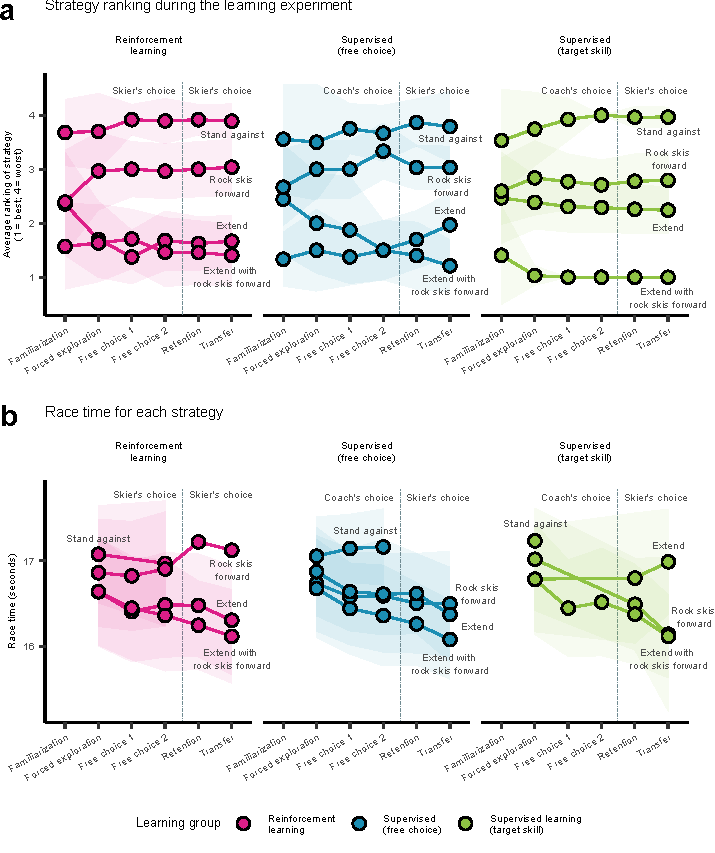
\includegraphics[]{figures/figure_ranking_average_3.pdf}
\caption{Strategy evaluations and effects. \textbf{a. }Average descriptive ranking of the four strategies per treatment group. Rankings range from 1 (best) to 4 (worst). For supervised (free choice) learning, the coach's ranking during the acquisition phase and the skier's ranking during the retention and transfer phases are plotted, reflecting the decision- maker for strategy selection. The circle represents the mean, and the ribbon indicates the standard deviation (SD). \textbf{b.} Average race time of the four strategies across the three treatment groups. The circle represents the mean, and the ribbon represents the SD. Note that all skiers tested the strategies during the forced exploration phase, but as the study progressed, there may have been fewer observations for some strategies. Consequently, the calculation of the mean might be heavily influenced by these observations. The mean race time was calculated by first determining each participant's average time for each strategy per session, followed by calculating the mean of these averages.}\label{fig: rank}
\end{figure}


\section{Discussion}

Learning to select effective strategies is a distinctive characteristic of expertise. Typically, these strategies come from a coach who imparts knowledge on which strategies to adopt. Here, we instead asked whether shifting the training strategy from direct instruction to evaluation can accelerate the development of expertise in skilled performers. To address this question, we developed four strategies with the potential to improve race time on flat sections in slalom and allocated ninety-eight skilled alpine ski racers to one of three treatment groups who learned the strategy choices in different ways. The skiers in the reinforcement learning group were tasked with finding the best of these strategies themselves using trial feedback for evaluation. The skiers in the supervised (free choice) learning group were assigned to a coach from the tested ski teams who selected a strategy for the skier and provided feedback on their execution. Finally, in the supervised (target skill) learning group, the skiers were assigned a current national team coach to coach in the 'extend with rock skis forward' skiing strategy — a technique we defined as the theoretically best strategy based on observations of elite skiers, simulations and theory. Overall, we found that reinforcement learning learned better than the supervised (free choice) learning group [usikker på om jeg skal ta med noe mer hva vi fant her faktisk?]

To begin, our findings that reinforcement learning improved more during acquisition and demonstrated greater retention than supervised (free choice) learning are in accordance with previous studies showing that reinforcement learning improves skill retention \cite{therrien_effective_2016, truong_error-based_2023, hasson_reinforcement_2015}. One suggested explanation for these findings is that reinforcement learning trains the slow-learning process that secures long-term learning \cite{huang_rethinking_2011}. The better race times in reinforcement learning also align with prior studies on the 'discovery learning' approach, where practice without explicit instruction yields better learning effects \cite{wulf_instructions_1997, hodges_learning_2001, hodges_role_1999}. We did, however, not find convincing evidence that reinforcement learning learned better than supervised (target skill) learning, although their race times were descriptively better during both acquisition and retention. The selection of strategy therefore appears to have played an important role, but we will offer a second account later in this discussion.

Contrary to our expectation, we did not find convincing evidence for improved transfer in the reinforcement learning group. One explanation for this is that reinforcement learning only improves learning in situations where rewards have been previously received \cite{robertson_memory_2018}, and aligns with \cite{hasson_reinforcement_2015} who found better retention but not transfer with reinforcement learning compared with supervised learning. It it possible that a more structured learning approach, where learners are exposed to frequent switches between situations, is necessary to grasp the task's structure and promote transfer \cite{braun_structure_2010}. Future research should possibly investigate the effect of structural learning. 

Our work sought to explain these differences in race times through the choice of strategies. We did not, however,  find convincing evidence that the reinforcement learning group selected the theoretical best or the individual skiers' estimated best strategy more often than the supervised (free choice) learning group. The choices were also characterized by a clear 'win-stay, lose-switch' signature in both groups, where the chooser opted to stick with choices that yielded good outcomes. However, despite significant descriptive differences favoring reinforcement learning, this pattern was not statistically significant either. An obvious explanation for this was the high coaching experience the coaches in the study possessed, as well as their access to the outcomes and undergoing considerable learning themselves. 

Despite the lack of convincing evidence that reinforcement learning selected the best strategy more often than supervised (free-choice) learning did, reinforcement learning had a lower expected cost (or regret) for skiers whose chosen strategies were suboptimal during retention. One explanation is that skiers in reinforcement learning gained better insight into the effectiveness of the strategies by objectively evaluating them during acquisition, which enabled them to choose strategies that did not adversely affect their times too much. This account cannot fully explain the group differences in race time, however. Reinforcement learning also improved more on the 'extend' strategy over the course of the sessions than supervised (free choice) learning. Given that this group was not assigned a coach to help them improve, it is likely that the reinforcement feedback increased motor vigor \cite{shadmehr_vigor_2020, pietro_mazzoni_why_2007, niv_normative_2006} when performing that strategy. Indeed, previous studies have shown that people make saccades \cite{takikawa_modulation_2002} and reach faster \cite{summerside_vigor_2018} toward targets paired with rewards than unpaired targets. Comments from a few coaches, who watched the retention and transfer from the sideline, mentioned that skiers in the reinforcement learning group used more forceful arm movements than skiers in the other groups, although the instructions did not explicitly tell them to do that.

The vigor perspective may also help explaining why reinforcement learning did not learn better than the supervised (target skill) learning group, as previous studies also have found that training with explicit knowledge boosts motor vigor much like the effect of reward itself \cite{anderson_rewards_2020, wong_explicit_2015}. It may therefore be that the getting information from a current national team coach that one strategy was best boosted the implicit motivation to perform this strategy well. 

A surprising and interesting discovery was that supervised (target skill) learning, in contrast to the reinforcement learning group, did not learn to cognitively dissociate the 'extend' and 'rock skis forward' strategies, despite big race time differences. This finding suggests that learners may miss potential learning by only being exposed to one strategy instead of a broader exploration of alternatives. Over time, such exploration could prove crucial in developing innovative strategies, as athletes cultivate a deeper comprehension of the relationship between their actions and performance outcomes \cite{ericsson_scientific_1998}. Future studies should investigate this learning further. 

The insights learned from our study suggest important implications for coaches when designing training sessions to improve skills. Based on our findings, coaches are advised to formulate strategies tailored to their respective sports and to aid learners in impartially evaluating these strategies. This pedagogical approach aligns with previous recommendations emphasizing the importance of fostering learners' cognitive representations to develop innovative solutions rather than merely imparting knowledge from a coach \cite{ericsson_scientific_1998}. These strategies may start out broadly for young athletes but should progressively become more focused as athletes advance in expertise. It is essential to clarify that we do not propose replacing traditional teaching methods with this approach but suggest integrating it as a supplementary tool to augment decision-making training.

Before practitioners embrace our recommendation to incorporate more strategy evaluation into their coaching practices, it is important to consider the practical significance of the effect size and its potential amplifying and counteracting mechanisms\cite{anvari_not_2023}. Notably, the estimated effect size during retention was smaller than our predefined smallest effect size of interest. This benchmark, however, was set for a longer slalom course and more training sessions than we could execute due to space and time constraints in the ski hall. Consequently, we exercise caution in outright dismissing its practical significance. However, our estimated effect size might be meaningful if we consider that our slalom course approximately equals one-third of a full slalom race course and that a slalom race consists of two runs. Therefore, the 0.12-second effect size could be scaled up by a factor of 6, but it is more realistic to assume that flat sections of a course constitute only one-third of the entire course. On this basis, the 0.12-second difference translates into an improved FIS world ranking of 27 positions for females and 65 for males, based on a median ranking of 600 in our sample (see Supplement Discussion \ref{supdiscussion}). This effect could be important for coaches, but we must remember that sports expertise involves cognitive decisions  \cite{mangalam_investigating_2023, krakauer_motor_2019}, such as switching from one strategy to another during a race. Our study did not capture such decisions because we focused on flat sections, only. Finally, the estimated effects would possibly been larger if the skiers in the reinforcement learning and supervised had performed the retention and transfer test in separate sessions with no information leakage. When we tested the skiers simultaneously allowed the skiers to observe each other, possibly diluting some of the effect. However, this decision was made to mirror the conditions of alpine competitions and gave us confidence that athletes experienced similar conditions during testing.


\subsection{Limitation of the study}

One limitation of the study is that we did not include motion capture of the skiers performing the strategies. Therefore, we do not know precisely what the skiers did when executing the strategies, other than verifying that they were able to perform the strategy satisfactorily during the famiration phase. However, we followed the recommendation to make discrete strategies. 

\section{Conclusion}
In conclusion, our data showed that reinforcement learning performed better than the standard coaching approach, although this learning did not transfer to a new slalom course. Only by informing coaches about what we believed to be the best strategy for improving race time on flats on slalom were we able to produce learning effects similar to those of reinforcement learning. However, these race times were still descriptively slower than the reinforcement learning. Always picking the correct strategy had as its own cost, however. The learner may not learn the causal structure supporting their performance, which might prevent them from developing truly intelligent solutions \cite{ericsson_scientific_1998}. Our findings corroborate previous research showing that reinforcement learning can be an important learning mechanism \cite{hasson_reinforcement_2015} and that it can be an important training strategy for training skilled performers \cite{lohse_errors_2019}.



\backmatter

\bmhead{Supplementary information}

If your article has accompanying supplementary file/s please state so here. 

Authors reporting data from electrophoretic gels and blots should supply the full unprocessed scans for key as part of their Supplementary information. This may be requested by the editorial team/s if it is missing.

Please refer to Journal-level guidance for any specific requirements.

\bmhead{Acknowledgements}

Acknowledgements are not compulsory. Where included they should be brief. Grant or contribution numbers may be acknowledged.

Please refer to Journal-level guidance for any specific requirements.

\section*{Declarations}

Some journals require declarations to be submitted in a standardised format. Please check the Instructions for Authors of the journal to which you are submitting to see if you need to complete this section. If yes, your manuscript must contain the following sections under the heading `Declarations':

\begin{itemize}
\item Funding
\item Conflict of interest/Competing interests (check journal-specific guidelines for which heading to use)
\item Ethics approval and consent to participate
\item Consent for publication
\item Data availability 
\item Materials availability
\item Code availability 
\item Author contribution
\end{itemize}

\noindent
If any of the sections are not relevant to your manuscript, please include the heading and write `Not applicable' for that section. 

%%===================================================%%
%% For presentation purpose, we have included        %%
%% \bigskip command. Please ignore this.             %%
%%===================================================%%
\bigskip
\begin{flushleft}%
Editorial Policies for:

\bigskip\noindent
Springer journals and proceedings: \url{https://www.springer.com/gp/editorial-policies}

\bigskip\noindent
Nature Portfolio journals: \url{https://www.nature.com/nature-research/editorial-policies}

\bigskip\noindent
\textit{Scientific Reports}: \url{https://www.nature.com/srep/journal-policies/editorial-policies}

\bigskip\noindent
BMC journals: \url{https://www.biomedcentral.com/getpublished/editorial-policies}
\end{flushleft}

\begin{appendices}

\section{Description of strategies}\label{sup_strategies}
This supplementary describes each strategy in more detail. 

The "stand against" strategy emphasized maintaining a stable stance against external forces without body extension along the body's longitudinal axis or rocking skis forward. This term is frequently used by Norwegian ski coaches when communicating with skiers to help them improve their race times. 

The "rock skis forward" strategy involves rocking the ski forward during the turning phase. This action effectively regulates the distribution of pressure over the skis. During the initiation and control phases of a turn, the pressure is generally shifted forward to bend the ski's forebody, increasing friction with the snow and enabling it to turn more sharply. However, at some point, during turn progression, the skier aims to stop turning and therefore shifts the pressure further back on the skis, thereby reducing turning and braking forces \cite{lemaster_skiers_1999, lemaster_ultimate_2010}. Investigations of elite alpine ski racers have shown that high performing skiers tend to rock skis more forward and pressure the back part of the ski for considerable longer time during a turn, than slower skiers \cite{reid_kinematic_2010, tjorhom_beskrivelse_2007, reid_alpine_2020}. To make the information more specific for the skiers, we communicated, that the maximum range of the rocking movement was about 30-50 centimeters from gate passage to completion of the turn, which is in correspondence with biomechanical evidence of elite ski racers \cite{reid_kinematic_2010}. 

The "extend" strategy involves extending the body from a laterally tilted position during the turn, closer to the turn's center of rotation. This pushing motion leads to more proper handling of a reservoir of energy available when skiers lower their bodies in the switch between turns. When skiers extend their bodies, while being laterally inclined in the slalom turn, they create ground reaction force. The radial component of the ground reaction force moving the center of mass closer to the center of rotation increases velocity, in accord with the principle of mechanical energy conservation \cite{lind_physics_2013}. Simulation studies of individuals extending their body in rollers or during carved slalom turns have shown that this movement can increase speed \cite{mote_accelerations_1983,luginbuhl_identification_2023}, and the effect has been observed in various ways with elite skiers during training and competition \cite{reid_kinematic_2010, magelssen_is_2022, supej_differential_2008}. 

Finally, "extend with rocking skis forward" was expected to be the best strategy combining the two effects from extending and rocking skis forward, and we therefore defined this as the theoretical best strategy. Simulations of skiers extending their bodies in the bottom of a roller have observed an additional effect of rocking the skis forward \cite{mote_accelerations_1983}


\section{Snow preparation}\label{sup_snowprep}
We dedicated a substantial amount of time and effort to prepare the hill for our learning experiment. Our primary objective was to ensure that the snow conditions were as identical and fair as possible for all participants. To achieve this, we collaborated closely with the SNØ facility’s staff and the coaches of the Norwegian Alpine Ski team. Together, we devised a comprehensive plan to achieve consistency before each group of skiers took to the slopes. This report will detail the steps we took to ensure the snow was ready for our skiers and provide insight into the reasoning behind our choices. The purpose of this supplementary note is to assist you in evaluating our study and to transparently document our commitment to delivering the best possible conditions for our skiers.

\subsection*{Ski group A}
About two weeks before testing Group A, new snow was created on the racing hill. The evening before data collection, machines groomed the racing hill (Fig. \ref{fig:snowprep}a:left). We then watered the hill and left it to freeze overnight to create a hard and firm surface (Fig. \ref{fig:snowprep}a:right). 

\subsection*{Ski group B}
Ski group B began testing the day after ski group A completed their testing. Once group A finished, we inspected the race hill(Fig. \ref{fig:snowprep}b:left), noticed some small holes, and decided to fill them before watering it again (Fig. \ref{fig:snowprep}b:right).  

\subsection*{Ski group C}
After ski group B, the race hill started getting icy, lacking grip in some areas. We were concerned that watering it again might worsen conditions, making it too challenging for skiers. Consequently, we opted to gently groom the hill with a machine and let the grooves set for a couple of days. See figure \ref{fig:snowprep}c for the result of this process.

\begin{figure}[H]
\centering
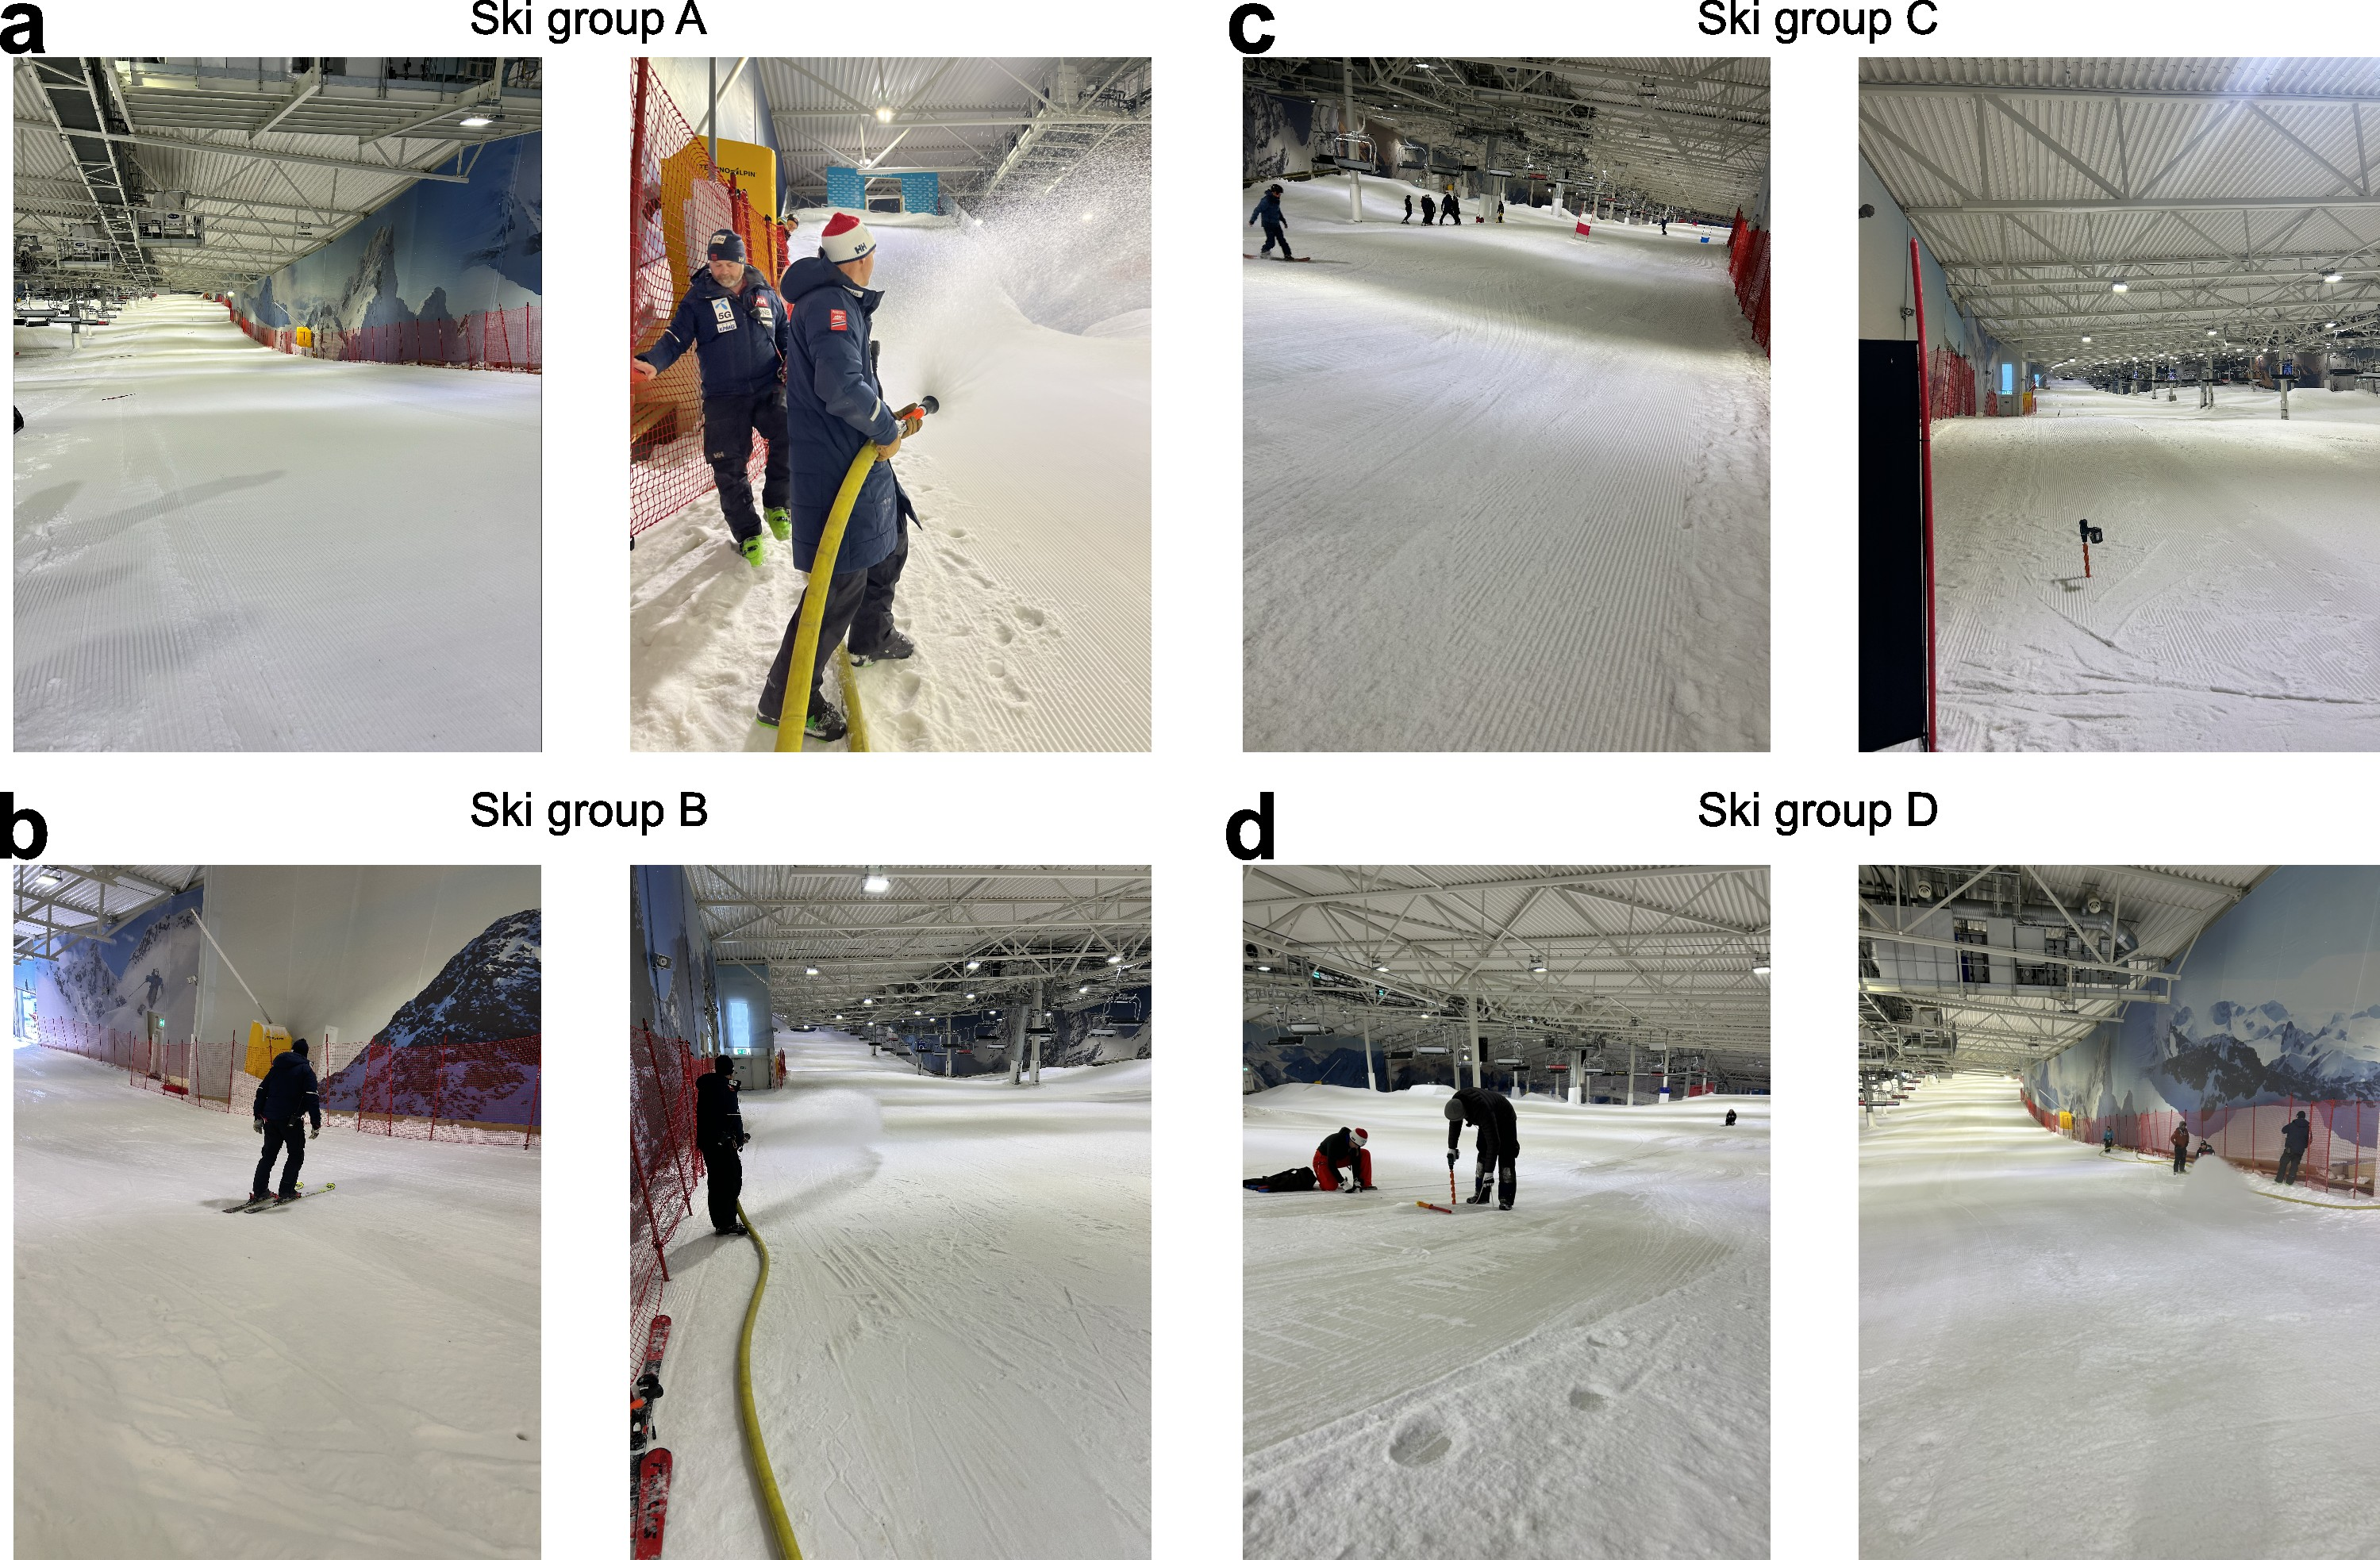
\includegraphics[width=\linewidth]{figures/figure_appendix_snowprep.jpg}
\caption{Images showing the hill preparation for the four ski groups. \textbf{a}. Shows the racing hill for ski group A. The left image displays the racing hill the evening before data collection after it was groomed. The right image shows the watering process for ski group A. \textbf{b}. Shows the racing hill for ski group B. The left image depicts the course inspection immediately after ski group A finished their testing. The right image shows the watering process for ski group B. Note that we did not groom the course this time, so in the image, you can see some uneven surfaces on the snow, which were evened out by watering it. \textbf{c}. Shows the racing hill for ski group C. The left image displays the hill after it was groomed and left overnight. The right image shows the same but from the bottom. \textbf{d}. Shows the racing hill for ski group D. The left image illustrates the hill for ski group C on their retention test. Note the icy surface, which was the reason why we produced new snow. The right image shows the watering process for ski group D. 
}
\label{fig:snowprep}
\end{figure}
 
\subsection*{Ski group D}
After Ski Group C, the race hill needed new snow because some areas had become icy, with minimal grip (Fig. ref{fig:snowprep}d:left)). Although the conditions were suitable for Ski Group C, they would not have worked for a new ski group undergoing testing. Consequently, we decided to produce new snow two days before Ski Group D started their training. This fresh snow was pushed into the racing hill the day before testing and groomed. Subsequently, we watered the hill and let it freeze overnight (Fig. \ref{fig:snowprep}d:right)



\section{Course setting}\label{sup_coursesetting}
We used a standard procedure to set the slalom courses, ensuring a fixed length and offset. First, we stretched a taut rope between two nails on either side of the ski hill. This rope helped us locate the exact starting line consistently from day to day. From the nail on the skier's right, we measured 6 meters into the slope. We did the same from a fixed point approximately 50 meters down the course, but here we measured 3.4 meters out. Then, we pulled a 50-meter-long measuring tape between the two points to establish the line down the hill   We chose a measuring tape over a rope because ropes tend to expand and contract when they get wet and dry, respectively (see Fig.\ref{fig:coursesetting}a for an image illustrating this process).

\begin{figure}[H]
\centering
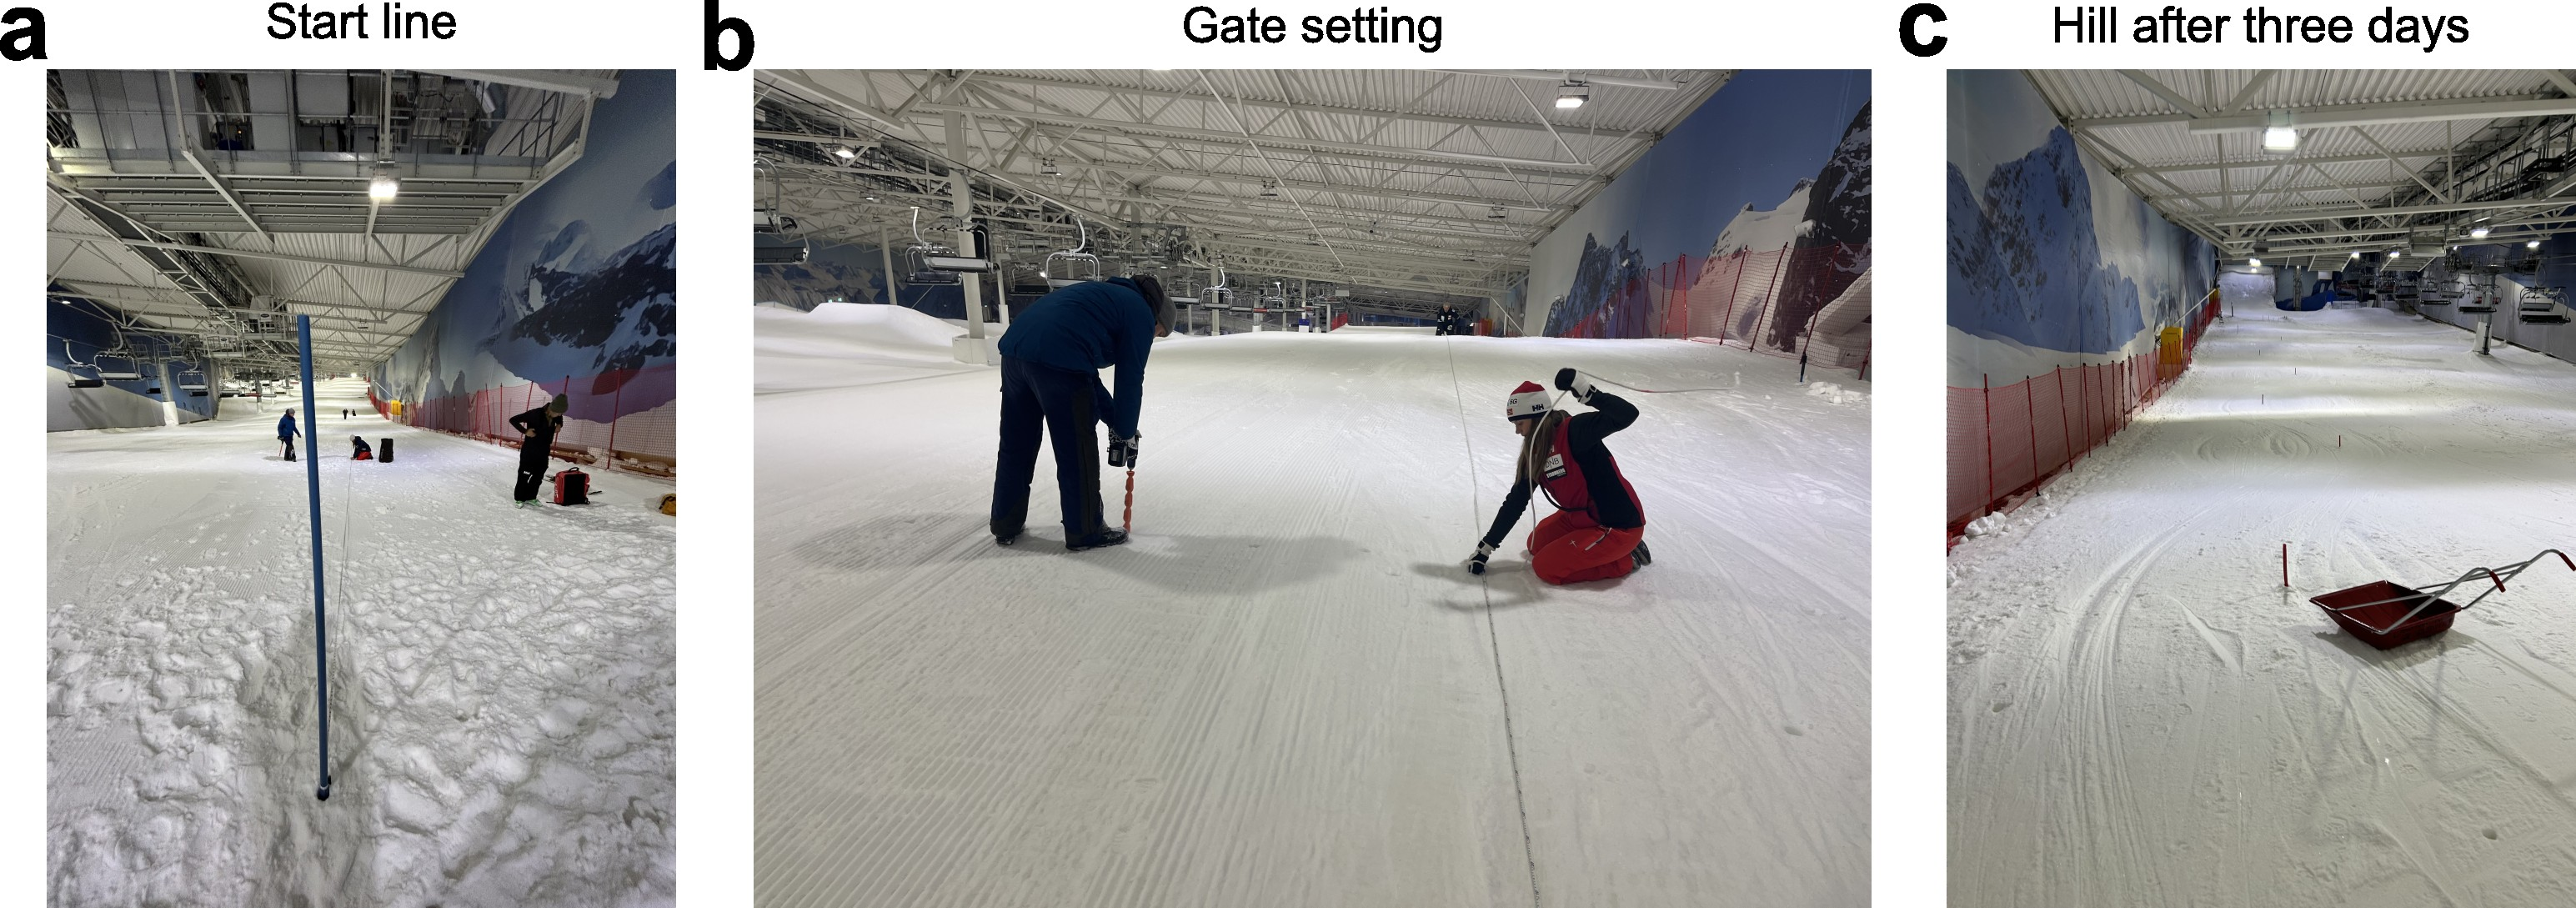
\includegraphics[width=\linewidth]{figures/figure_appendix_coursesetting.jpg}
\caption{Images showing the procedure for course setting. \textbf{a}. The image illustrates the process of establishing the straight reference line down the hill. The long blue gate is positioned 6 meters from the nail on the skier's right. \textbf{b}. This image showcases the gate-setting method. A white rope is secured to the reference line with a carabiner hook, and a marker on the rope indicates a distance of 1.9 meters for placing the gate. \textbf{c}. The image reveals the tracks left behind by a group of skiers that was tested
}
\label{fig:coursesetting}
\end{figure}
 

Once the 50-meter straight line was established, we laid out a rope segment attached to a carabiner hooked onto the long rope. We moved this segment 1.9 meters out from the rope in one turn and 0 meters in the other, with a 10-meter vertical space. This ensured that the course followed a straight line down the slope and was set with the correct offset (see figure\ref{fig:coursesetting}b for an image illustrating this process). Once all the gates along the 50-meter measurement tape were set, we used a new fixation point down the slope and continued down the course. We practiced this procedure several times before the experiment, and the variation in course setting was a maximum of 10 cm at the end of the course.

Due to wear and tear on the trails, we opted to shift the course laterally or rotate it, depending on the situation. With the exception of one skiing group, we followed the following practice. On day 1, we set the course as described above. On day 2, we rotated the course so that the first turn went in the opposite direction of day 1. On the third day, we shifted the course closer to the wall on skiers' right (see figure \ref{fig:coursesetting}c for an image showing the tracks in the hill left after a skigroup had completed the experiment). 


\section{Coach setup}
We set up three coach stations in the finishing area for the supervised learning groups, one for each coach. The space between the coaches was approximately 3 to 5 meters. We used wall dividers to prevent information leakage between the coaches. In addition, the background noise in the ski hall was generally high, and it was difficult to perceive information without standing close to the person. The supervised (target skill) learning coach was behind the two other coaches to prevent the other coaches from seeing what he did. Each coach had a monitor where they could see their own (but not the other) skiers' race.

\begin{figure}[H]
\centering
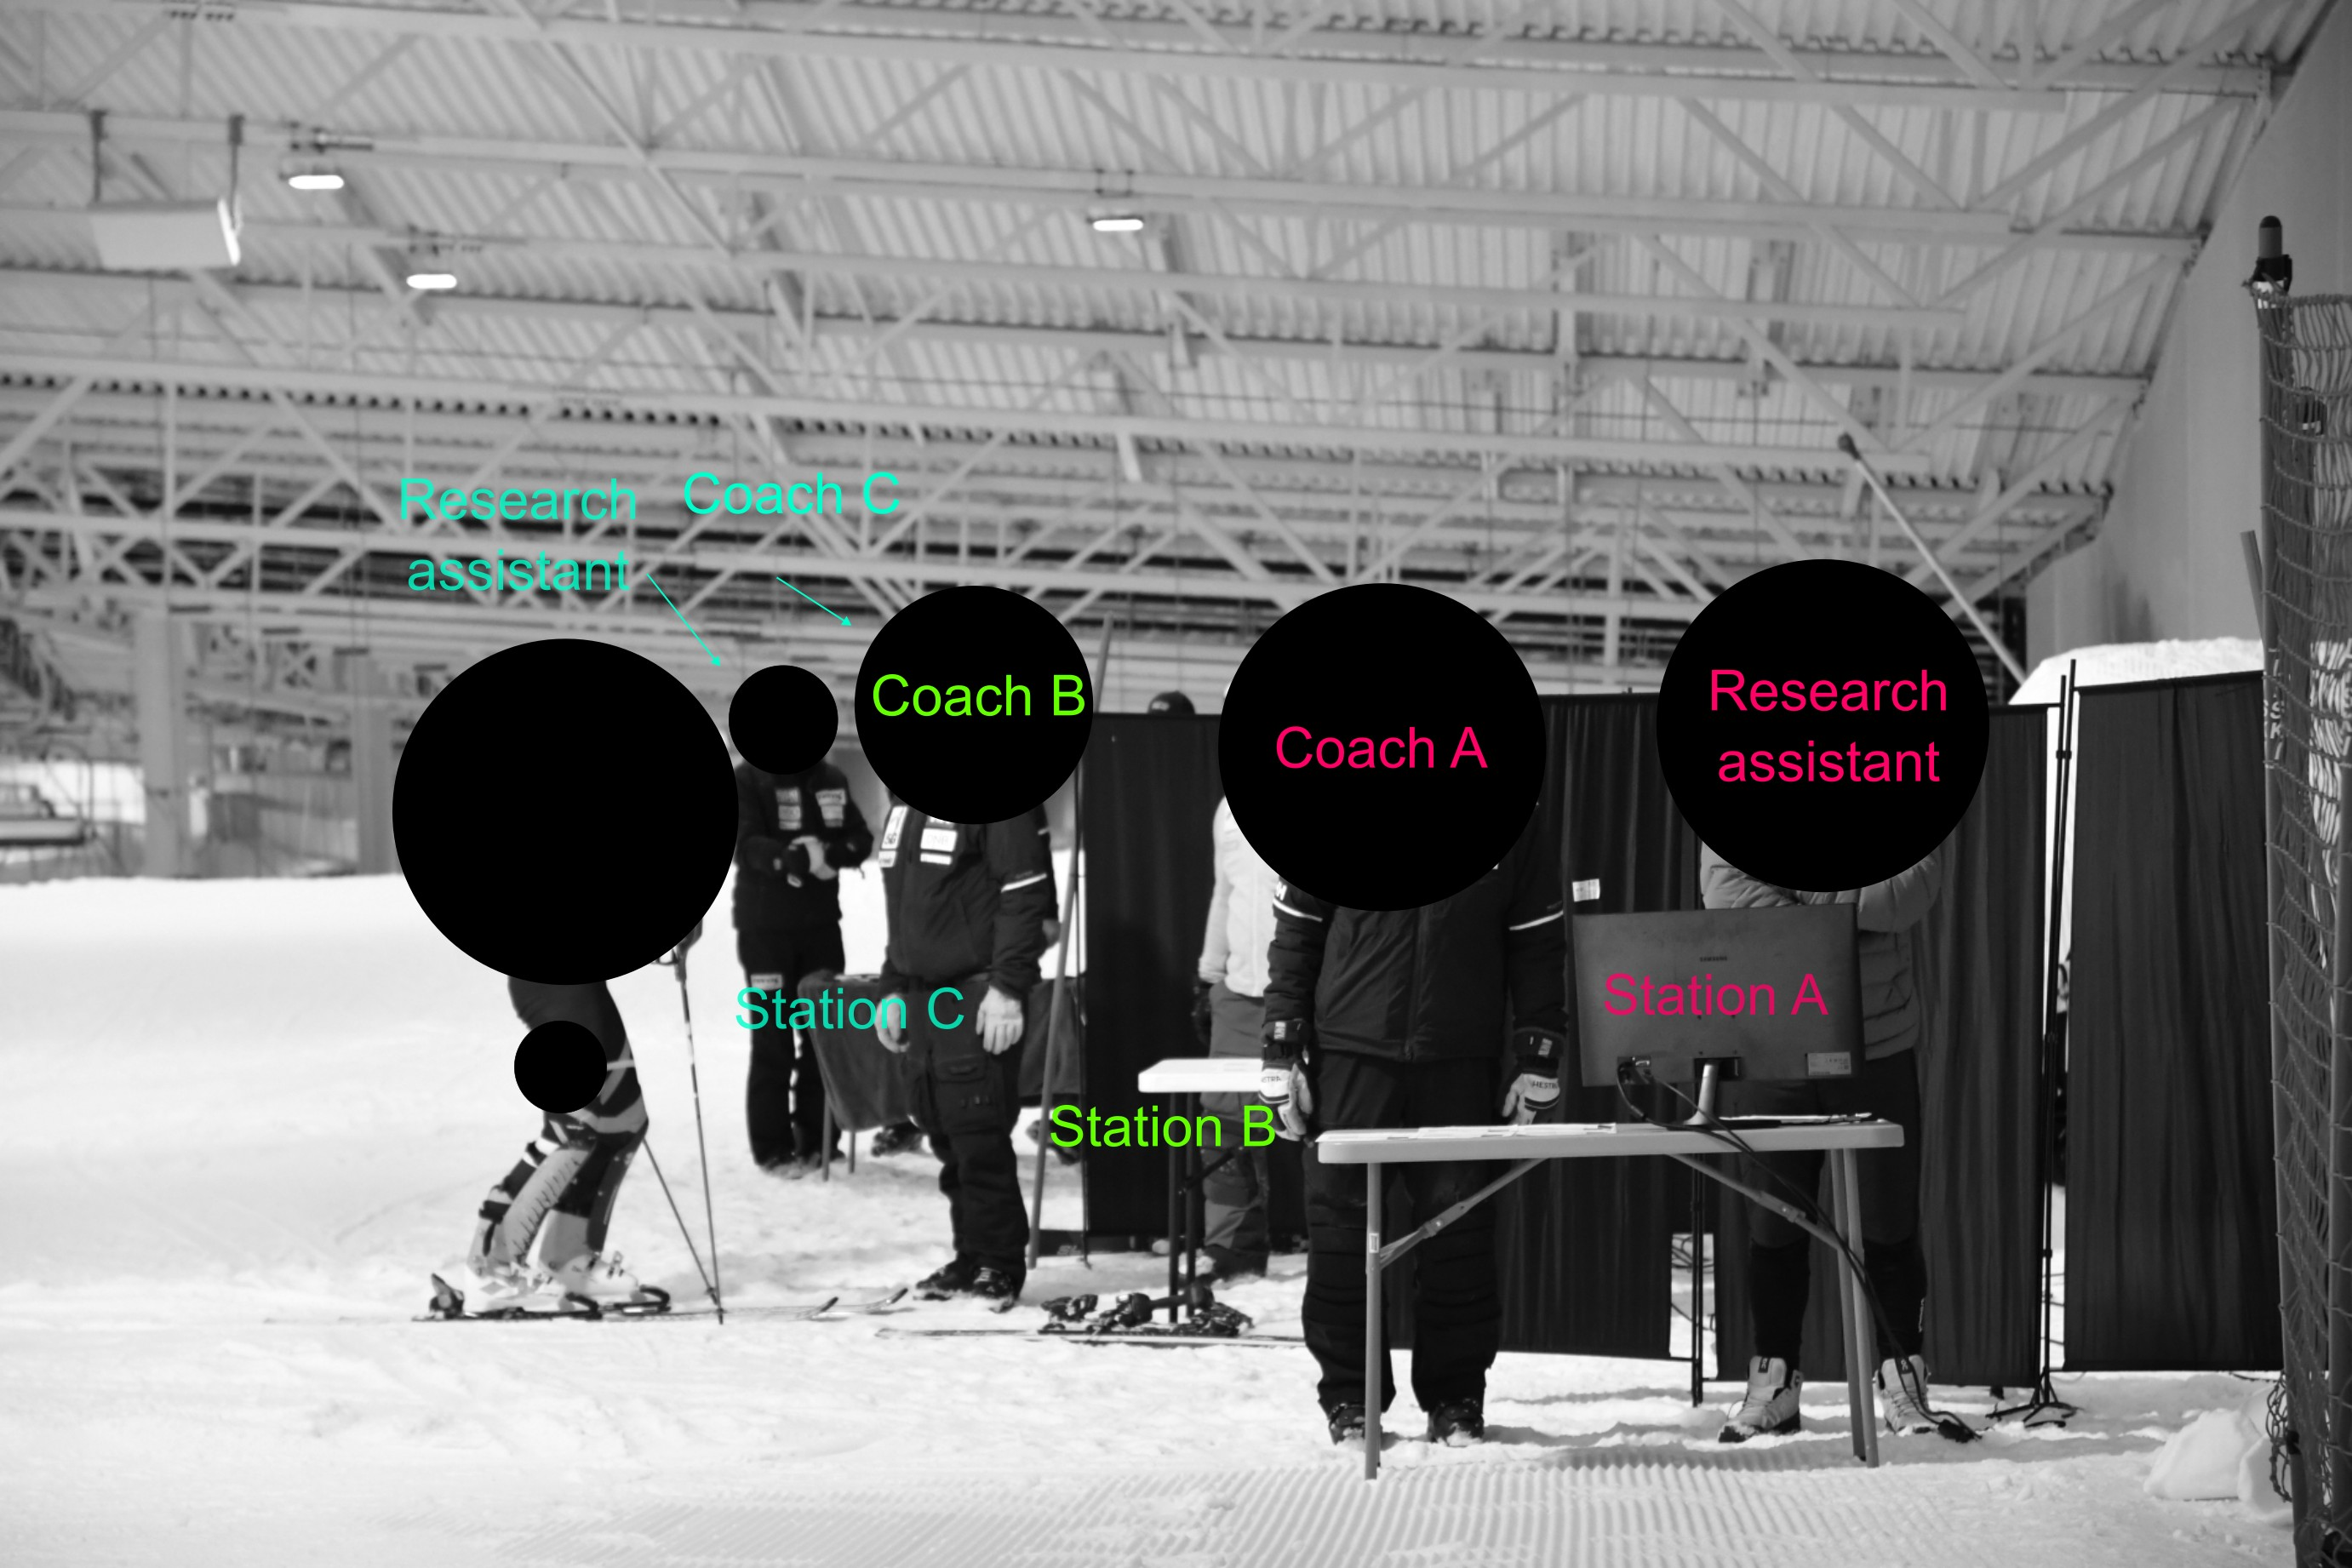
\includegraphics[width=\linewidth]{figures/figure_appendix_coachstation.jpg}
\caption{Images shows the setup in the finish area
}
\label{fig:coachstation}
\end{figure}
 




\section{Supplementary Table}

\subsection{Race time}

\begin{table}[h!]
\caption{Race time: Estimated improvement across sessions in acquisition}\label{table_racetime_acquisition_change}
\centering
\begin{tabular}{lrrrrrrrr}
  \hline
 Term & Estimate & SE & df & CI & t & p \\ 
  \hline
 (Intercept) & 16.62 & 0.13 & 3.93 & 16.27-16.97 & 132.69 &  $<$  0.001 \\ 
   supervised (free choice) & 0.14 & 0.13 & 85.83 & -0.12-0.39 & 1.04 &    0.299 \\ 
   supervised (target skill) & 0.14 & 0.13 & 85.82 & -0.12-0.40 & 1.10 &    0.276 \\ 
  reinforcement learning : free choice 1 & -0.38 & 0.03 & 91.63 & -0.45--0.31 & -10.82 &  $<$  0.001 \\ 
   supervised (free choice) : free choice 1 & -0.30 & 0.03 & 93.47 & -0.37--0.23 & -8.96 &  $<$  0.001 \\ 
   supervised (target skill) : free choice 1 & -0.50 & 0.03 & 91.95 & -0.57--0.44 & -15.08 &  $<$  0.001 \\ 
   reinforcement learning : free choice 2 & -0.45 & 0.05 & 95.16 & -0.54--0.36 & -9.99 &  $<$  0.001 \\ 
   supervised (free choice) : free choice 2 & -0.31 & 0.04 & 96.39 & -0.39--0.22 & -7.17 &  $<$  0.001 \\ 
   supervised (target skill) : free choice 2 & -0.43 & 0.04 & 96.20 & -0.52--0.35 & -10.07 &  $<$  0.001 \\ 
   sd(Intercept) & 0.51 &  &  &  &  &  &  \\ 
   cor(Intercept,free choice 1) & -0.03 &  &  &  &  &  &  \\ 
   cor(Intercept,free choice 2) & 0.23 &  &  &  &  &  &  \\ 
   sd(free choice 1) & 0.15 &  &  &  &  &  &  \\ 
   cor(free choice 1,free choice 2) & 0.73 &  &  &  &  &  &  \\ 
  sd(free choice 2) & 0.22 &  &  &  &  &  &  \\ 
   sd(Intercept) & 0.23 &  &  &  &  &  &  \\ 
   sd(Observation) & 0.21 &  &  &  &  &  &  \\ 
   \hline
\end{tabular}
\footnotetext{Formula: racetime ~ treatment / session + (1 $|$skigroup) + (1 + session $|$ skigroup:skier)}
\end{table}


\begin{table}[h!]
\caption{Race time: Estimated difference between groups during acquisition}\label{table_racetime_acquisition_groupdifference}
\centering
\begin{tabular}{lrrrrrrrr}
  \hline
 Term & Estimate & SE & df & CI & t & p \\ 
  \hline
 (Intercept) & 16.62 & 0.13 & 3.93 & 16.27-16.97 & 132.68 &  $<$  0.001 \\ 
 free choice 1 & -0.39 & 0.02 & 92.32 & -0.43--0.35 & -20.09 &  $<$  0.001 \\ 
  free choice 2 & -0.40 & 0.03 & 95.89 & -0.45--0.35 & -15.74 &  $<$  0.001 \\ 
  forced exploration : supervised (free choice) & 0.06 & 0.13 & 92.73 & -0.20-0.32 & 0.48 &    0.631 \\ 
  free choice 1 : supervised (free choice) & 0.14 & 0.13 & 86.15 & -0.11-0.39 & 1.11 &   0.272 \\ 
  free choice 2 : supervised (free choice) & 0.20 & 0.14 & 78.00 & -0.08-0.49 & 1.43 &   0.157 \\ 
  forced exploration : supervised (target skill) & 0.18 & 0.13 & 92.66 & -0.08-0.44 & 1.37 &   0.174 \\ 
  free choice 1 : supervised (target skill) & 0.05 & 0.13 & 86.12 & -0.20-0.31 & 0.43 &   0.672 \\ 
  free choice 2 : supervised (target skill) & 0.19 & 0.14 & 78.02 & -0.09-0.48 & 1.37 &   0.176 \\ 
  sd(Intercept) & 0.51 &  &  &  &  &    \\ 
  cor(Intercept).free choice 1 & -0.03 &  &  &  &  &    \\ 
  cor(Intercept).free choice 2 & 0.23 &  &  &  &  &    \\ 
  sd(free choice 1) & 0.15 &  &  &  &  &    \\ 
  cor(free choice 1,free choice 2) & 0.73 &  &  &  &  &   \\ 
  sd(free choice 2) & 0.22 &  &  &  &  &    \\ 
  sd(Intercept) & 0.23 &  &  &  &  &   \\ 
  sd(Observation) & 0.21 &  &  &  &   &  \\ 
   \hline
\end{tabular}
\footnotetext{Formula: racetime ~ session / treatment + (1 $|$skigroup) + (1 + session $|$ skigroup:skier)}
\end{table}










\subsection{Strategy choice}








\begin{table}[ht]
\caption{Probability change across sessions}\label{strategychoice_theorybest_change}
\begin{tabular}{llrrrrrrr}
  \hline
 Contrast & Treatment & Estimate & SE & df & CI & z & p \\ 
  \hline
  free choice 2 - free choice 1 & rl & 0.02 & 0.06 & Inf & -0.11-0.14 & 0.26 &   0.791 \\ 
  retention - free choice 1 & rl & 0.07 & 0.07 & Inf & -0.07-0.21 & 0.96 &   0.339 \\ 
  retention - free choice 2 & rl & 0.05 & 0.07 & Inf & -0.09-0.19 & 0.72 &    0.469 \\ 
  transfer - free choice 1 & rl & 0.18 & 0.07 & Inf & 0.04-0.32 & 2.58 &    0.010 \\ 
  transfer - free choice 2 & rl & 0.16 & 0.07 & Inf & 0.03-0.30 & 2.34 &    0.019 \\ 
  transfer - retention & rl & 0.11 & 0.08 & Inf & -0.04-0.27 & 1.42 &    0.155 \\ 
  free choice 2 - free choice 1 & slfc & 0.08 & 0.06 & Inf & -0.04-0.21 & 1.32 &    0.188 \\ 
  retention - free choice 1 & slfc & 0.31 & 0.07 & Inf & 0.18-0.44 & 4.59 &  $<$  0.001 \\ 
  retention - free choice 2 & slfc & 0.23 & 0.07 & Inf & 0.09-0.36 & 3.31 &  $<$  0.001 \\ 
  transfer - free choice 1 & slfc & 0.36 & 0.07 & Inf & 0.23-0.50 & 5.33 &  $<$  0.001 \\ 
  transfer - free choice 2 & slfc & 0.28 & 0.07 & Inf & 0.14-0.42 & 4.02 &  $<$  0.001 \\ 
  transfer - retention & slfc & 0.05 & 0.06 & Inf & -0.07-0.18 & 0.85 &    0.396 \\ 
   \hline
\end{tabular}
\footnotetext{Formula: glmer(chosetheorybest treatment * session + (1 $|$ skigroup/skier).}
\footnotetext{rl = reinforcement learning; slfc = supervised (free choice) learning}
\end{table}

\newpage

\begin{table}[ht]
\caption{Predicted probability difference between groups}\label{strategychoice_theorybest_groupdiff}
\begin{tabular}{llrrrrrrl}
  \hline
 Contrast & Session & Estimate & SE & df & CI & z & p \\ 
  \hline
rl minus slfc & free choice 1 & 0.01 & 0.13 & Inf & -0.24-0.27 & 0.11 &  0.911 \\ 
rl minus slfc & free choice 2 & -0.05 & 0.13 & Inf & -0.31-0.20 & -0.39 &   0.693 \\ 
rl minus slfc & retention & -0.23 & 0.13 & Inf & -0.48-0.03 & -1.75 &  0.079 \\ 
rl minus slfc & transfer & -0.17 & 0.12 & Inf & -0.40-0.07 & -1.41 &  0.159 \\ 
   \hline
\end{tabular}
\footnotetext{Formula: glmer(chosetheorybest treatment * session + (1 $|$ skigroup/skier).}
\footnotetext{rl = reinforcement learning; slfc = supervised (free choice) learning.}
\end{table}




\begin{table}[h!]
\caption{Strategy choice: Predicted probability change in probability of choosing the individual skier's estimated best strategy}\label{table_strategychoice_estimatedbest_change}
\centering
\begin{tabular}{lllrrrrrrr}
  \hline
  Contrast & Treatment & Estimate & SE & df & CI & z & p \\ 
  \hline
 free choice 2 - free choice 1 & rl & 0.20 & 0.06 & Inf & 0.09-0.32 & 3.39 &  $<$  0.001 \\ 
   retention - free choice 1 & rl & 0.13 & 0.06 & Inf & 0.00-0.26 & 2.02 &    0.043 \\ 
  retention - free choice 2 & rl & -0.07 & 0.06 & Inf & -0.19-0.04 & -1.25 &    0.213 \\ 
  transfer - free choice 1 & rl & 0.21 & 0.06 & Inf & 0.09-0.34 & 3.30 &  $<$  0.001 \\ 
  transfer - free choice 2 & rl & 0.01 & 0.05 & Inf & -0.09-0.11 & 0.18 &    0.854 \\ 
   transfer - retention & rl & 0.08 & 0.06 & Inf & -0.04-0.20 & 1.31 &    0.190 \\ 
   free choice 2 - free choice 1 & slfc & 0.09 & 0.06 & Inf & -0.03-0.21 & 1.48 &    0.140 \\ 
   retention - free choice 1 & slfc & 0.21 & 0.07 & Inf & 0.08-0.34 & 3.11 &    0.002 \\ 
   retention - free choice 2 & slfc & 0.12 & 0.06 & Inf & -0.00-0.24 & 1.88 &    0.060 \\ 
   transfer - free choice 1 & slfc & 0.23 & 0.07 & Inf & 0.10-0.36 & 3.39 &  $<$  0.001 \\ 
   transfer - free choice 2 & slfc & 0.14 & 0.06 & Inf & 0.02-0.26 & 2.21 &    0.027 \\ 
   transfer - retention & slfc & 0.02 & 0.06 & Inf & -0.09-0.13 & 0.35 &    0.727 \\ 
   \hline
\end{tabular}
\footnotetext{Formula: glmer(choseestimatedbest treatment * session + (1 $|$ skigroup/skier).}
\footnotetext{rl = reinforcement learning; slfc = supervised (free choice) learning}
\end{table}


\begin{table}[h!]
\caption{Strategy choice: Predicted probability difference of choosing the individual skier's estimated best strategy at each session}\label{table_strategychoice_estimatedbest_groupdiff}
\centering
\begin{tabular}{rllrrrrrrl}
  \hline
 Contrast & Session & Estimate & SE & df & CI & z & p \\ 
  \hline
 rl minus slfc & block2 & 0.01 & 0.12 & Inf & -0.22-0.24 & 0.12 &    0.904 \\ 
   rl minus slfc & block3 & 0.13 & 0.10 & Inf & -0.06-0.32 & 1.30 &    0.194 \\ 
   rl minus slfc & retention & -0.06 & 0.10 & Inf & -0.26-0.14 & -0.61 &    0.544 \\ 
  rl minus slfc & transfer & 0.00 & 0.09 & Inf & -0.17-0.17 & 0.00 &    0.999 \\ 
   \hline
\end{tabular}
\footnotetext{Formula: glmer(choseestimatedbest treatment * session + (1 $|$ skigroup/skier).}
\footnotetext{rl = reinforcement learning; slfc = supervised (free choice) learning}
\end{table}


\subsection{Strategy evaluations}

\begin{table}[h!]
\caption{Strategy evaluation: Estimated differences between strategy ranking during forced exploration}\label{table_strategyevaluation_diffstrategy}
\centering
\begin{tabular}{lrrrrrrr}
  \hline
 Term & Estimate & SE & CI & t & p \\ 
  \hline
 (Intercept) & 2.50 & 0.03 & 2.44-2.56 & 85.64 &  $<$  0.001 \\ 
 slfc & 0.00 & 0.08 & -0.16-0.16 & 0.00 &    1.000 \\ 
 slts & 0.00 & 0.05 & -0.11-0.11 & 0.00 &    1.000 \\ 
 ranktime & 0.00 & 0.01 & -0.02-0.02 & 0.00 &    1.000 \\ 
 rl : b & -1.72 & 0.11 & -1.94--1.50 & -15.47 &  $<$  0.001 \\ 
 slfc : b & -1.43 & 0.19 & -1.81--1.05 & -7.38 &  $<$  0.001 \\ 
 slts : b & -1.20 & 0.11 & -1.41--0.99 & -11.32 &  $<$  0.001 \\ 
 rl : c & -1.05 & 0.11 & -1.27--0.83 & -9.42 &  $<$  0.001 \\ 
 slfc : c & -0.70 & 0.19 & -1.08--0.32 & -3.60 &  $<$  0.001 \\ 
 slts : c & -0.95 & 0.11 & -1.16--0.74 & -8.94 &  $<$  0.001 \\ 
  rl : d & -2.06 & 0.11 & -2.28--1.84 & -18.49 &  $<$  0.001 \\ 
  slfc : d & -2.09 & 0.19 & -2.47--1.71 & -10.77 &  $<$  0.001 \\ 
  slts : d & -2.41 & 0.11 & -2.61--2.20 & -22.67 &  $<$  0.001 \\ 
  slfc : ranktime & -0.00 & 0.02 & -0.04-0.04 & -0.00 &    1.000 \\ 
  slts : ranktime & -0.00 & 0.02 & -0.04-0.04 & -0.00 &    1.000 \\ 
  rl : b : ranktime & -0.15 & 0.04 & -0.22--0.07 & -3.95 &  $<$  0.001 \\ 
  slfc : b : ranktime & -0.12 & 0.05 & -0.22--0.02 & -2.45 &    0.014 \\ 
  slts : b : ranktime & -0.13 & 0.04 & -0.20--0.06 & -3.65 &  $<$  0.001 \\ 
  rl : c : ranktime & 0.05 & 0.04 & -0.03-0.12 & 1.21 &    0.225 \\ 
  slfc : c : ranktime & -0.01 & 0.05 & -0.11-0.09 & -0.27 &    0.791 \\ 
  slts : c : ranktime & -0.06 & 0.04 & -0.13-0.01 & -1.78 &    0.076 \\ 
  rl : d : ranktime & -0.09 & 0.04 & -0.17--0.02 & -2.51 &    0.012 \\ 
  slfc : d : ranktime & -0.09 & 0.05 & -0.19-0.01 & -1.85 &    0.065 \\ 
  slts : d : ranktime & -0.15 & 0.04 & -0.22--0.08 & -4.18 &  $<$  0.001 \\ 
   \hline
\end{tabular}
\footnotetext{Formula: lm(value ~ treatment/strategy * ranktime)}
\footnotetext{rl = reinforcement learning; slfc = supervised (free choice) learning, slts = supervised (target skill) learning, b="extend", c="rock skis forward", d="extend with rock skis forward"}
\end{table}


\begin{table}[h!]
\caption{Strategy evaluation: Estimated differences between groups on strategy ranking during forced exploration}\label{table_strategyevaluation_diffgroup}
\centering
\begin{tabular}{lrrrrrrr}
  \hline
 Term & Estimate & SE & CI & t & p \\ 
  \hline
 (Intercept) & 2.50 & 0.03 & 2.44-2.56 & 85.64 &  $<$  0.001 \\ 
   b & -1.45 & 0.08 & -1.61--1.29 & -17.58 &  $<$  0.001 \\ 
   c & -0.90 & 0.08 & -1.06--0.74 & -10.88 &  $<$  0.001 \\ 
   d & -2.18 & 0.08 & -2.35--2.02 & -26.46 &  $<$  0.001 \\ 
   ranktime & -0.00 & 0.01 & -0.02-0.02 & -0.00 &    1.000 \\ 
   a : slfc & -0.15 & 0.16 & -0.46-0.16 & -0.96 &    0.340 \\ 
   b : slfc & 0.14 & 0.16 & -0.17-0.45 & 0.87 &    0.385 \\ 
   c : slfc & 0.20 & 0.16 & -0.11-0.51 & 1.26 &    0.209 \\ 
   d : slfc & -0.19 & 0.16 & -0.50-0.13 & -1.17 &    0.242 \\ 
   a : slts & -0.07 & 0.11 & -0.28-0.15 & -0.63 &    0.531 \\ 
   b : slts & 0.45 & 0.11 & 0.24-0.67 & 4.17 &  $<$  0.001 \\ 
   c : slts & 0.03 & 0.11 & -0.18-0.24 & 0.29 &    0.772 \\ 
   d : slts & -0.42 & 0.11 & -0.63--0.20 & -3.83 &  $<$  0.001 \\ 
   b : ranktime & -0.13 & 0.02 & -0.18--0.09 & -5.56 &  $<$  0.001 \\ 
   c : ranktime & -0.01 & 0.02 & -0.06-0.04 & -0.43 &    0.665 \\ 
   d : ranktime & -0.11 & 0.02 & -0.16--0.06 & -4.65 &  $<$  0.001 \\ 
   a : slfc : ranktime & 0.01 & 0.04 & -0.08-0.10 & 0.19 &    0.847 \\ 
   b : slfc : ranktime & 0.03 & 0.04 & -0.05-0.12 & 0.73 &    0.465 \\ 
   c : slfc : ranktime & -0.05 & 0.04 & -0.14-0.04 & -1.13 &    0.259 \\ 
   d : slfc : ranktime & 0.01 & 0.04 & -0.08-0.10 & 0.21 &    0.837 \\ 
   a : slts : ranktime & 0.04 & 0.04 & -0.03-0.11 & 1.00 &    0.317 \\ 
   b : slts : ranktime & 0.05 & 0.04 & -0.02-0.13 & 1.48 &    0.140 \\ 
   c : slts : ranktime & -0.07 & 0.04 & -0.14--0.00 & -1.97 &    0.049 \\ 
   d : slts : ranktime & -0.02 & 0.04 & -0.09-0.05 & -0.50 &    0.615 \\ 
   \hline
\end{tabular}
\footnotetext{Formula: lm(value ~ strategy / treatment * ranktime)}
\footnotetext{rl = reinforcement learning; slfc = supervised (free choice) learning, slts = supervised (target skill) learning, b="extend", c="rock skis forward", d="extend with rock skis forward"}
\end{table}



\begin{table}[h!]
\caption{Strategy evaluation: Estimated slope for each strategy across session}\label{table_strategyevaluation_slopestrategy}
\centering
\begin{tabular}{llrrrrrr}
  \hline
 Term & Estimate & SE & CI & t & p \\ 
  \hline
(Intercept) & 2.50 & 0.03 & 2.44-2.56 & 85.64 &  $<$  0.001 \\ 
  slfc & 0.00 & 0.08 & -0.16-0.16 & 0.00 &    1.000 \\ 
  slts & 0.00 & 0.05 & -0.11-0.11 & 0.00 &    1.000 \\ 
  b & -1.45 & 0.08 & -1.61--1.29 & -17.58 &  $<$  0.001 \\ 
  c & -0.90 & 0.08 & -1.06--0.74 & -10.88 &  $<$  0.001 \\ 
  d & -2.18 & 0.08 & -2.35--2.02 & -26.46 &  $<$  0.001 \\ 
  slfc : b & 0.29 & 0.22 & -0.15-0.73 & 1.29 &    0.197 \\ 
  slts : b & 0.52 & 0.15 & 0.22-0.82 & 3.39 &  $<$  0.001 \\ 
  slfc : c & 0.35 & 0.22 & -0.09-0.79 & 1.56 &    0.118 \\ 
  slts : c & 0.10 & 0.15 & -0.20-0.40 & 0.65 &    0.517 \\ 
  slfc : d & -0.03 & 0.22 & -0.47-0.41 & -0.15 &    0.879 \\ 
  slts : d & -0.35 & 0.15 & -0.65--0.05 & -2.26 &    0.024 \\ 
rl : a : ranktime & 0.05 & 0.03 & -0.00-0.10 & 1.86 &    0.064 \\ 
slfc : a : ranktime & 0.06 & 0.04 & -0.01-0.13 & 1.61 &    0.107 \\ 
slts : a : ranktime & 0.09 & 0.03 & 0.04-0.13 & 3.40 &  $<$  0.001 \\ 
rl : b : ranktime & -0.10 & 0.03 & -0.15--0.05 & -3.73 &  $<$  0.001 \\ 
slfc : b : ranktime & -0.07 & 0.04 & -0.14-0.00 & -1.85 &    0.065 \\ 
slts : b : ranktime & -0.04 & 0.03 & -0.09-0.00 & -1.77 &    0.077 \\ 
rl : c : ranktime & 0.09 & 0.03 & 0.04-0.15 & 3.57 &  $<$  0.001 \\ 
slfc : c : ranktime & 0.04 & 0.04 & -0.03-0.11 & 1.24 &    0.216 \\ 
slts : c : ranktime & 0.02 & 0.03 & -0.03-0.07 & 0.89 &    0.376 \\ 
rl : d : ranktime & -0.04 & 0.03 & -0.10-0.01 & -1.70 &    0.090 \\ 
slfc : d : ranktime & -0.04 & 0.04 & -0.11-0.03 & -1.00 &    0.317 \\ 
slts : d : ranktime & -0.06 & 0.03 & -0.11--0.01 & -2.51 &    0.012 \\ 
   \hline
\end{tabular}
\footnotetext{Formula: lm(value ~  treatment * strategy / ranktime)}
\footnotetext{rl = reinforcement learning; slfc = supervised (free choice) learning, slts = supervised (target skill) learning, b="extend", c="rock skis forward", d="extend with rock skis forward"}
\end{table}









\section{Supplementary discussion}\label{supdiscussion}
To convert race time to FIS World Ranking, we assumed that each second corresponded to a 7-point FIS. We could then multiply by 0.12 * 7 to find the difference in FIS points. Then, we used the median rank in our sample and calculated what this difference corresponded to in the World Ranking. We performed this analysis for both females and men. Due to confidentiality, we do not want to say which FIS list we used for this conversion. If the reader thinks 7 points is too small or large, then we welcome the reader to change this number up or down. We only used this conversion to help readers evaluating the effect. 









%%=============================================%%
%% For submissions to Nature Portfolio Journals %%
%% please use the heading ``Extended Data''.   %%
%%=============================================%%

%%=============================================================%%
%% Sample for another appendix section			       %%
%%=============================================================%%

%% \section{Example of another appendix section}\label{secA2}%
%% Appendices may be used for helpful, supporting or essential material that would otherwise 
%% clutter, break up or be distracting to the text. Appendices can consist of sections, figures, 
%% tables and equations etc.

\end{appendices}

%%===========================================================================================%%
%% If you are submitting to one of the Nature Portfolio journals, using the eJP submission   %%
%% system, please include the references within the manuscript file itself. You may do this  %%
%% by copying the reference list from your .bbl file, paste it into the main manuscript .tex %%
%% file, and delete the associated \verb+\bibliography+ commands.                            %%
%%===========================================================================================%%

\bibliography{sn-bibliography}% common bib file
%% if required, the content of .bbl file can be included here once bbl is generated
%%\input sn-article.bbl


\end{document}
